\chapter{Experimentos e Resultados}
\label{cap:resultados}

\section{Configuração Experimental}
\label{sec:configuracao_experimental}

Os experimentos realizados neste trabalho buscaram avaliar a eficácia da abordagem proposta, que combina curriculum learning e self-play para o treinamento de agentes no ambiente de futebol de robôs. Para garantir uma avaliação consistente e comparativa, foi estabelecida uma configuração experimental padronizada, detalhada nesta seção.

\subsection{Hardware Utilizado}

Todos os experimentos foram executados em um ambiente computacional de alto desempenho, com especificações adequadas para treinamento de aprendizado por reforço distribuído. A configuração de hardware incluiu:

\begin{itemize}
    \item Processador: AMD Ryzen 7 7700x com 16 núcleos virtuais
    \item Memória RAM: 32GB DDR5
    \item GPU: NVIDIA GeForce RTX 3090 com 24GB de memória VRAM
    \item Armazenamento: SSD NVMe de 2TB para leitura e escrita rápidas de checkpoints
\end{itemize}

A utilização de hardware especializado foi fundamental para viabilizar o treinamento distribuído com múltiplos trabalhadores paralelos, acelerando significativamente o processo experimental.

\subsection{Parâmetros de Treinamento}

Os parâmetros de treinamento foram cuidadosamente selecionados para garantir um equilíbrio entre eficiência computacional e qualidade do aprendizado, tentando mater o mais próximo possível do padrão utilizado no artigo original. Os principais parâmetros utilizados incluem:

\begin{itemize}
    \item \textbf{Algoritmo}: Proximal Policy Optimization (PPO) 
    \item \textbf{Taxa de aprendizado}: 0.0004 - Define o tamanho dos passos durante a otimização, controlando a velocidade do aprendizado
    \item \textbf{Função de ativação}: ReLU - Função não-linear que permite à rede neural aprender padrões complexos, zerando valores negativos
    \item \textbf{Arquitetura da rede neural}: Fully Connected com camadas [300, 200, 100] - Estrutura da rede neural com três camadas ocultas totalmente conectadas
    \item \textbf{Batch size}: 96000 (calculado como workers x envs x fragment) - Quantidade total de amostras processadas em cada iteração de treinamento
    \item \textbf{Mini-batch size}: 24000 (batch/4) - Subdivisão do batch para processamento em lotes menores, otimizando o uso de memória
    \item \textbf{Número de workers}: 12 (ambientes paralelos) - Quantidade de processos paralelos executando o ambiente de simulação
    \item \textbf{Ambientes por workers}: 4 - Número de ambientes simultâneos gerenciados por cada worker
    \item \textbf{Gamma}: 0.99 - Fator de desconto que determina a importância de recompensas futuras
    \item \textbf{Lambda}: 0.95 - Parâmetro de equilíbrio entre viés e variância no cálculo da vantagem generalizada
    \item \textbf{Coeficiente de entropia}: 0.01 - Incentiva a exploração ao adicionar aleatoriedade na política
    \item \textbf{Clip param}: 0.2 - Limita o tamanho das atualizações da política para evitar mudanças muito grandes
    \item \textbf{Iterações SGD}: 8 - Número de passos de otimização realizados em cada batch de dados
\end{itemize}

No caso específico do curriculum learning, foram configurados dois estágios progressivos, com parâmetros específicos para cada um, conforme detalhado no Capítulo 3. A taxa de promoção entre estágios foi estabelecida em 80\% de sucesso em uma janela de 100 episódios.

\subsection{Tempo de Treinamento}

O tempo total de treinamento para cada experimento foi medido em termos de horas de execução na configuração de hardware utilizada. A Figura \ref{fig:tempo_treinamento} apresenta uma comparação dos tempos de treinamento para as diferentes abordagens implementadas.

\begin{figure}[H]
    \centering
    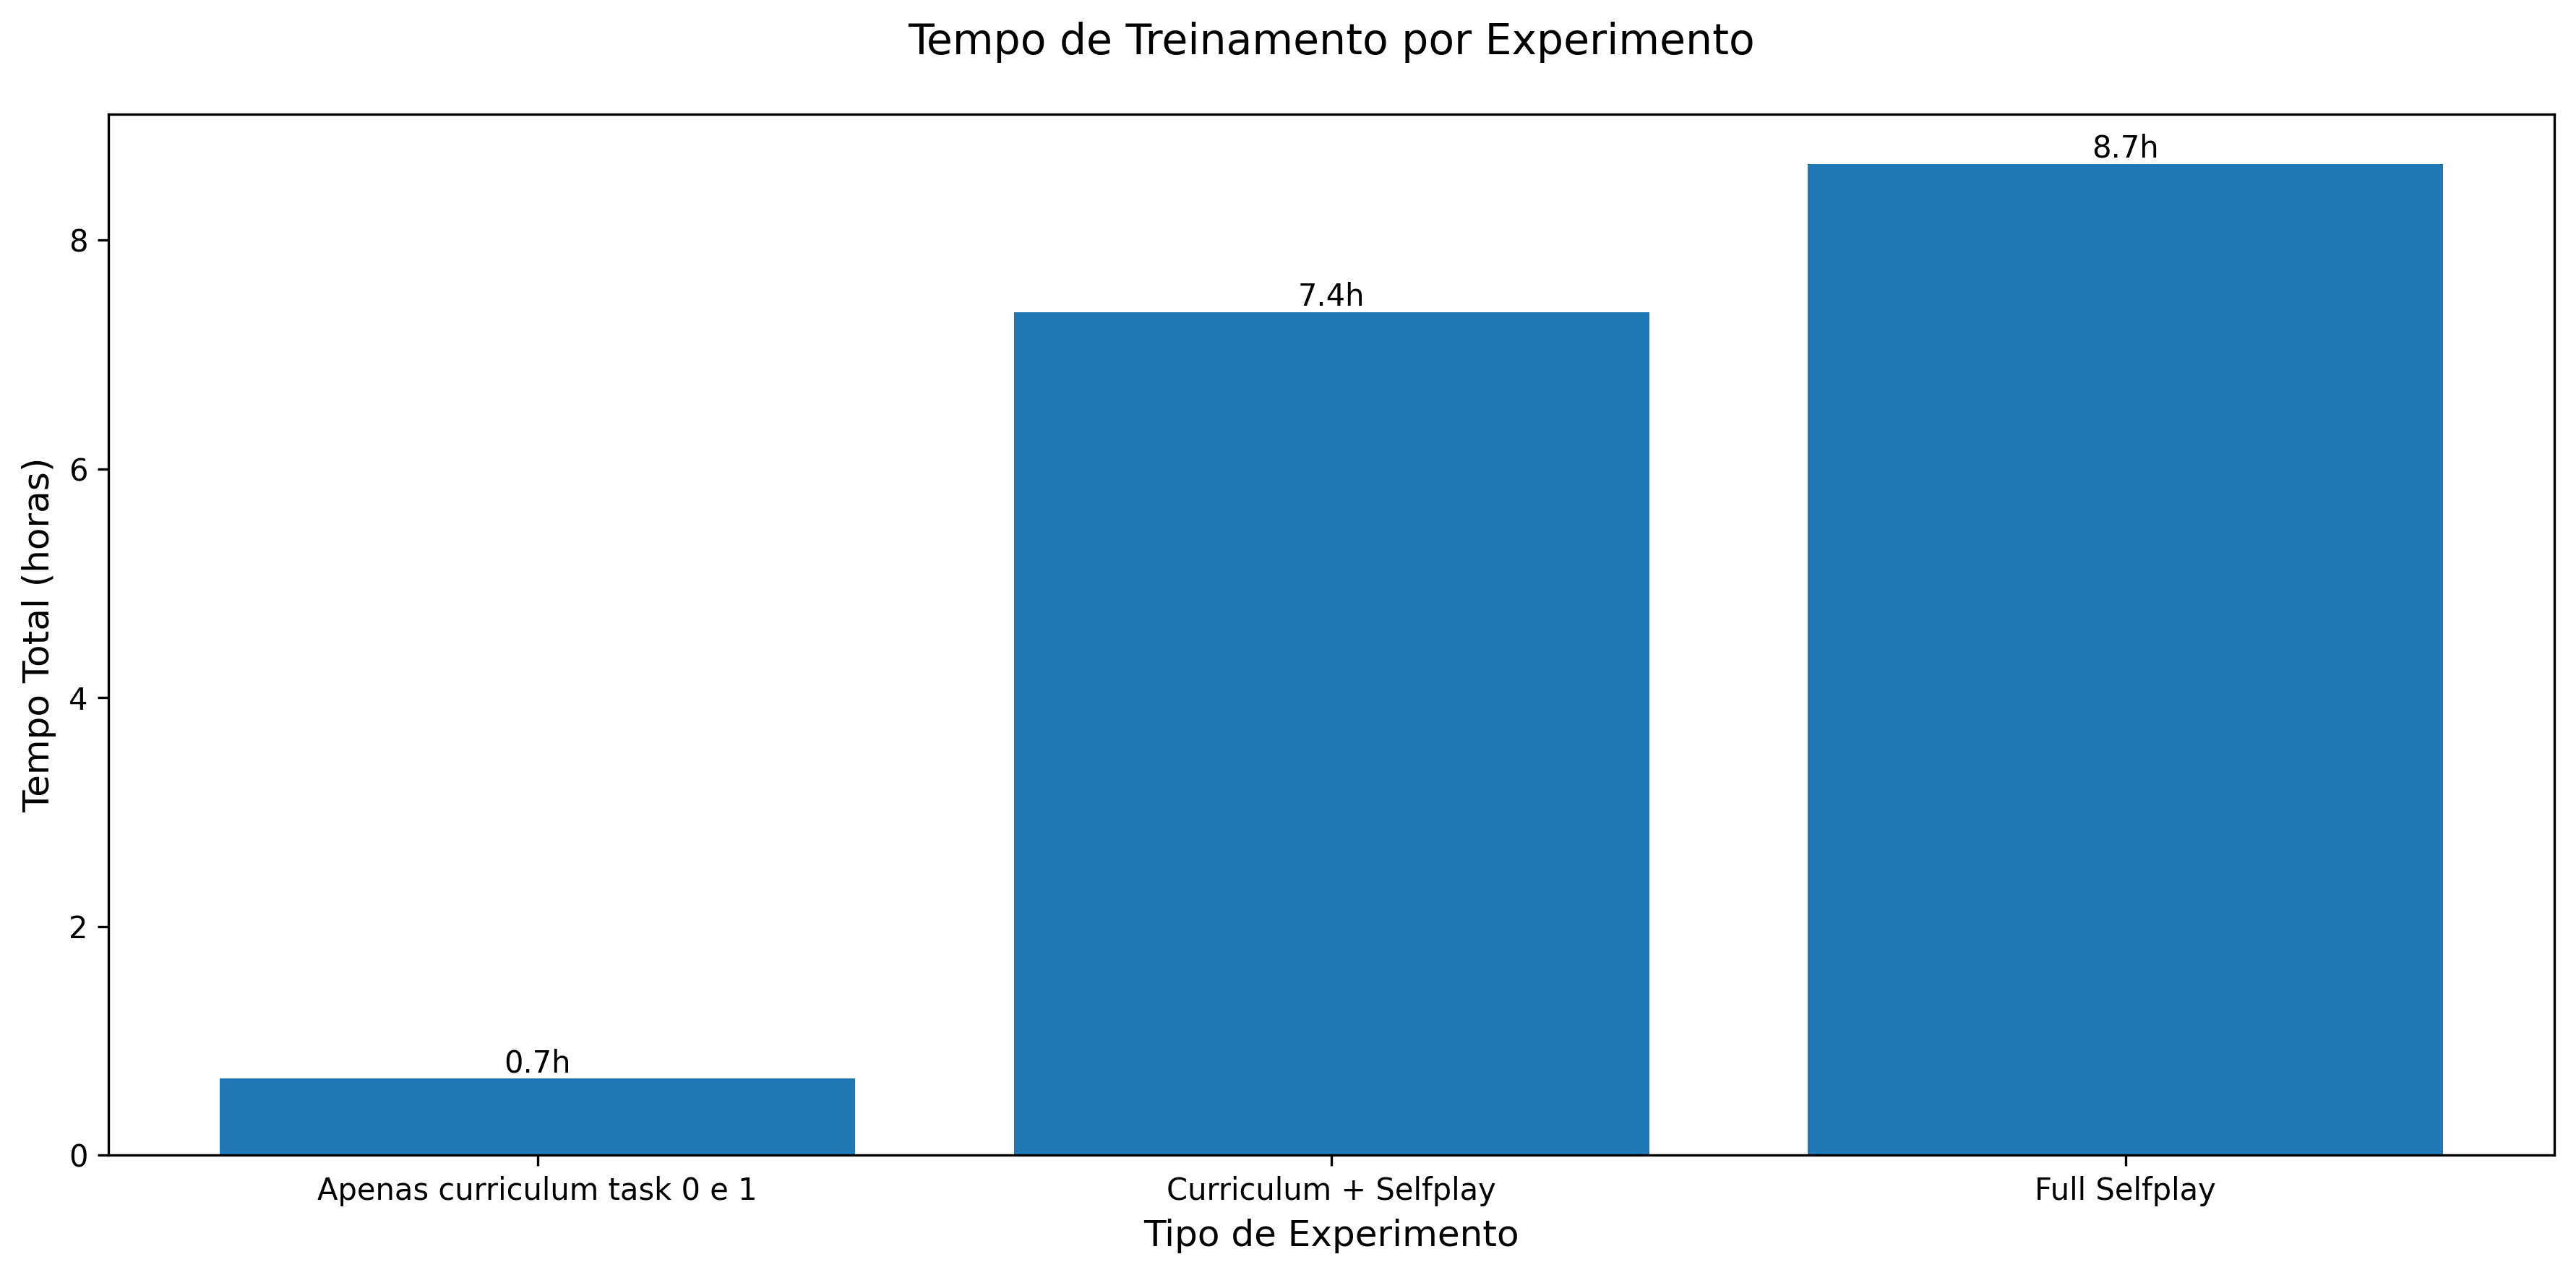
\includegraphics[width=0.9\textwidth]{fig/graficos_trabalho/graficos_experimentos/graficos_tempo_treino/tempo_treinamento.png}
    \caption{Comparação do tempo total de treinamento em horas para cada abordagem experimental}
    \label{fig:tempo_treinamento}
\end{figure}

A análise dos tempos de treinamento revela diferenças significativas entre as abordagens:

\begin{itemize}
    \item \textbf{Apenas curriculum (tasks 0 e 1)}: Aproximadamente 0,4 horas (24 minutos)
    \item \textbf{Curriculum + Self-play}: Aproximadamente 7,4 horas
    \item \textbf{Full Self-play (lado amarelo)}: Aproximadamente 12,1 horas
    \item \textbf{Full Self-play (lado azul)}: Aproximadamente 12,4 horas
\end{itemize}

Estas diferenças nos tempos de treinamento refletem a complexidade e a natureza de cada abordagem. O treinamento exclusivo com curriculum tasks é significativamente mais rápido, pois envolve ambientes mais simples e objetivos bem definidos. A abordagem combinada (curriculum + self-play) apresenta um tempo de treinamento intermediário, demonstrando uma vantagem de eficiência em relação ao self-play tradicional.

É interessante notar que a abordagem de full self-play para ambos os lados (azul e amarelo) exige aproximadamente o mesmo tempo de treinamento, com uma pequena variação que pode ser atribuída a flutuações nas condições de execução. No entanto, ambas requerem aproximadamente 66\% mais tempo que a abordagem combinada (curriculum + self-play).

Esta é uma observação particularmente relevante do ponto de vista prático, pois indica que além de proporcionar resultados superiores (conforme demonstrado nas seções anteriores), a abordagem combinada também oferece uma vantagem significativa em termos de eficiência computacional, reduzindo o tempo necessário para desenvolver agentes com desempenho competitivo.

A maior eficiência da abordagem combinada pode ser atribuída ao fato de que as habilidades fundamentais desenvolvidas durante o curriculum permitem que o agente aproveite melhor a fase de self-play, convergindo mais rapidamente para políticas efetivas.

\section{Análise Comparativa}
\label{sec:analise_comparativa}

Para avaliar a eficácia da abordagem proposta, realizamos uma análise comparativa entre o modelo treinado apenas com self-play (baseline) e o modelo treinado com a combinação de curriculum learning e self-play (modelo proposto). Esta análise abrange diversas métricas relevantes para o domínio do futebol de robôs.

\subsection{Evolução da Recompensa}

A análise da evolução da recompensa média ao longo do treinamento oferece insights valiosos sobre o processo de aprendizagem dos agentes. A Figura \ref{fig:episode_reward} apresenta esta evolução para ambas as abordagens.

\begin{figure}[H]
    \centering
    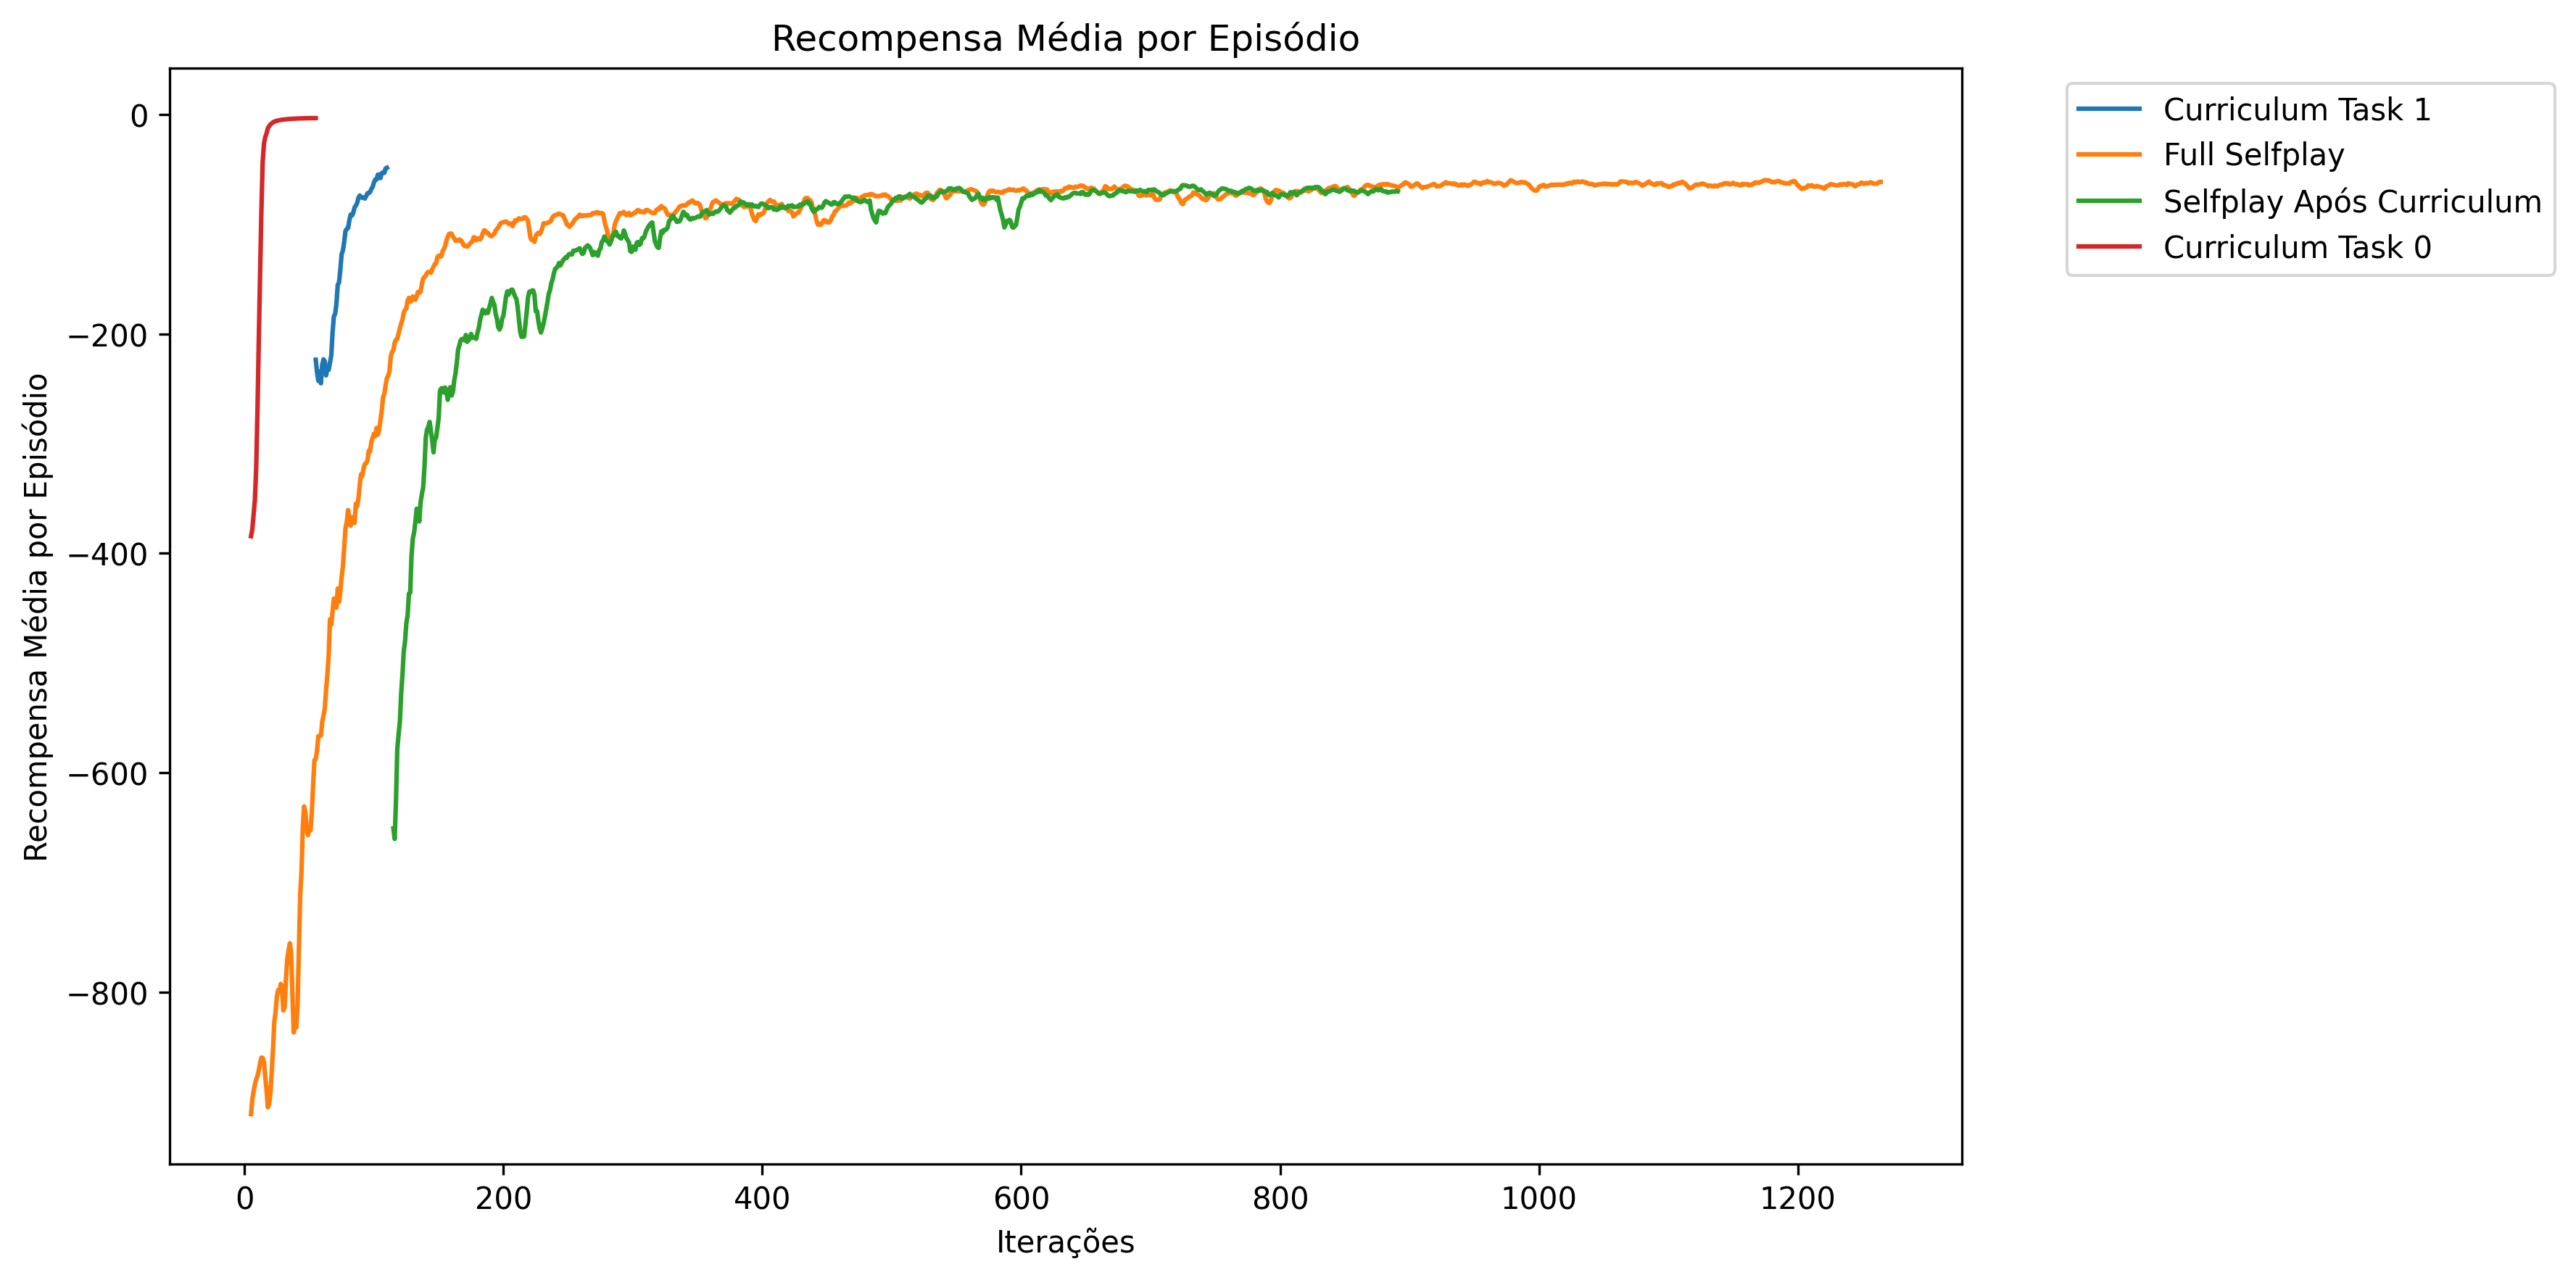
\includegraphics[width=0.8\textwidth]{fig/graficos_trabalho/graficos_experimentos/geral/episode_reward_mean.png}
    \caption{Evolução da recompensa média por episódio ao longo do treinamento}
    \label{fig:episode_reward}
\end{figure}

O gráfico revela que o modelo treinado com curriculum learning apresenta um crescimento mais acelerado da recompensa nas fases iniciais do treinamento. Esta vantagem inicial é atribuída à aprendizagem estruturada de habilidades fundamentais durante os estágios do curriculum. Embora ambas as abordagens apresentem convergência em termos de recompensa acumulada, o modelo proposto atinge níveis equivalentes com menos timesteps de treinamento, sugerindo maior eficiência no processo de aprendizagem.

Nota-se também que o modelo proposto apresenta menor variabilidade na curva de recompensa, indicando maior estabilidade durante o processo de treinamento.

\subsection{Desempenho Ofensivo}

O desempenho ofensivo dos agentes foi avaliado principalmente através da análise da média de gols marcados por episódio. A Figura \ref{fig:goals_blue_comparison} apresenta a evolução desta métrica ao longo do treinamento para ambas as abordagens.

\begin{figure}[H]
    \centering
    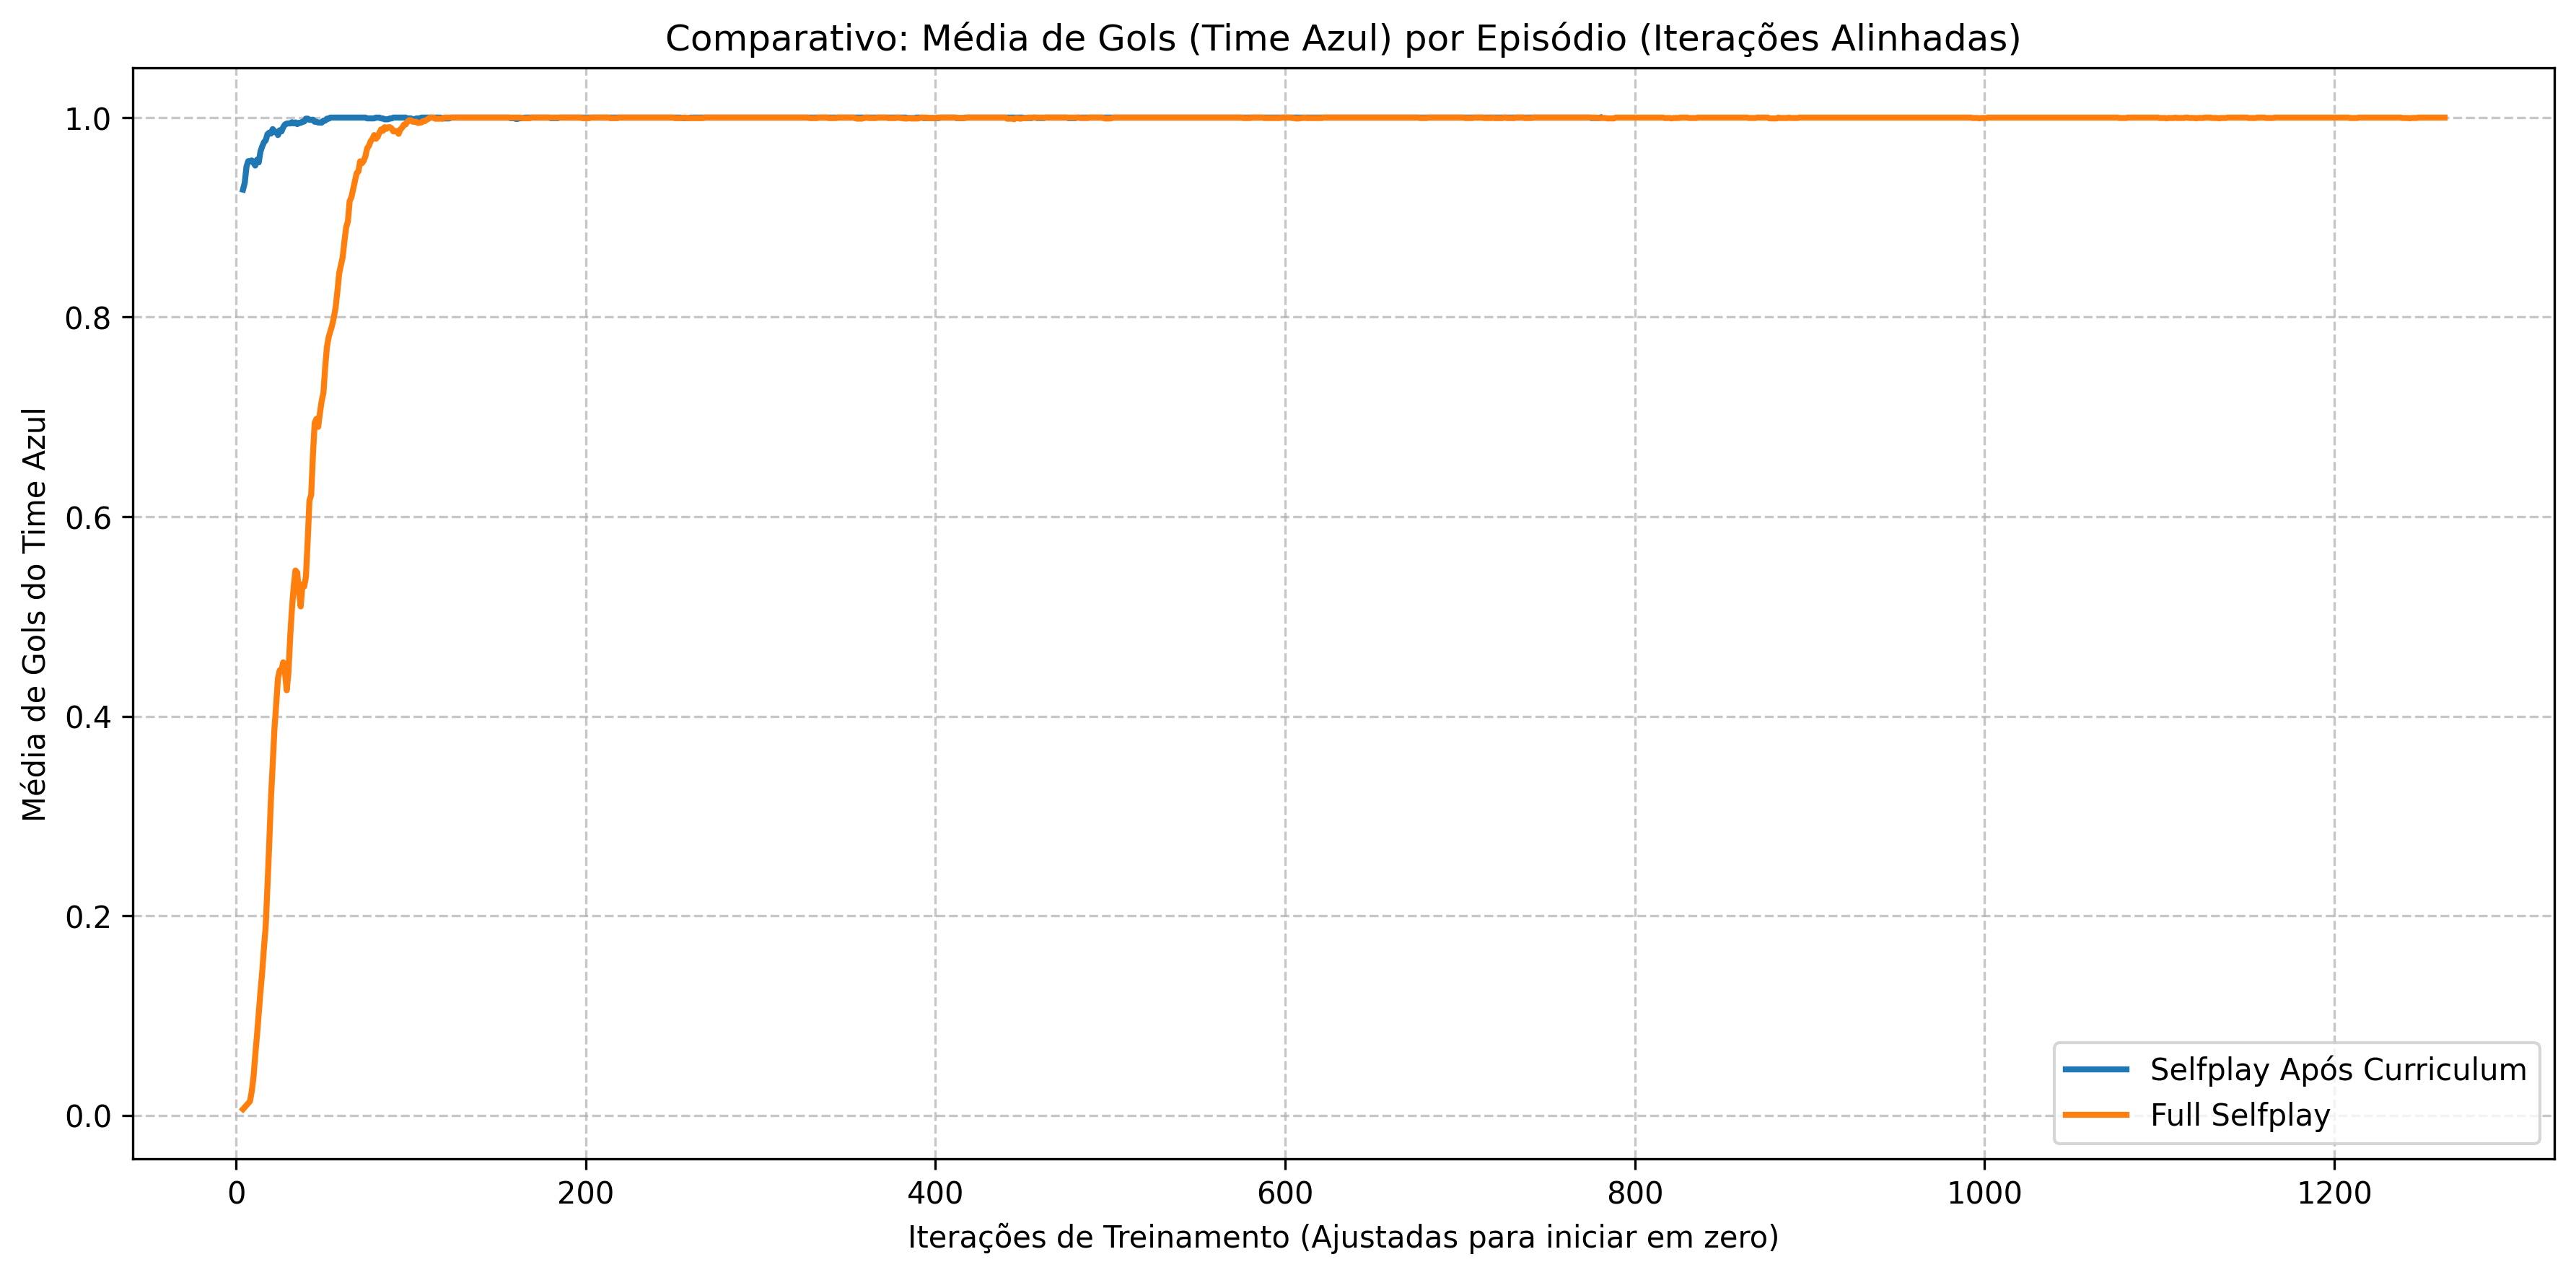
\includegraphics[width=0.95\textwidth]{fig/graficos_trabalho/graficos_experimentos/geral/comparativo_gols_azul_alinhado.png}
    \caption{Comparativo da média de gols do time azul por episódio com iterações alinhadas entre as abordagens Selfplay após Curriculum e Full Selfplay}
    \label{fig:goals_blue_comparison}
\end{figure}

A análise comparativa do gráfico revela padrões interessantes na evolução da capacidade ofensiva dos agentes. Ambas as abordagens apresentam uma progressão crescente na capacidade de marcar gols, atingindo valores próximos a 1 gol por episódio. No entanto, observam-se diferenças significativas no processo de aprendizado:

\begin{itemize}
    \item \textbf{Velocidade de convergência}: O Selfplay após Curriculum (linha azul) atinge o patamar de 1 gol por episódio muito mais rapidamente, convergindo em aproximadamente 100 iterações, enquanto o Full Selfplay (linha laranja) requer cerca de 150 iterações para alcançar o mesmo desempenho.
    
    \item \textbf{Fase inicial}: Nas primeiras iterações, o Selfplay após Curriculum já começa com uma vantagem significativa, demonstrando que as habilidades adquiridas durante a fase de curriculum proporcionam um ponto de partida mais avançado para o desenvolvimento ofensivo.
    
    \item \textbf{Estabilidade}: Ambas as abordagens eventualmente atingem estabilidade na média de gols, mas o Selfplay após Curriculum apresenta menor variabilidade na fase de convergência, indicando um processo de aprendizado mais consistente.
\end{itemize}

Esta comparação com iterações alinhadas evidencia de forma clara uma vantagem significativa da abordagem proposta: ao iniciar o self-play com agentes já treinados em tarefas fundamentais através do curriculum, obtém-se uma aceleração substancial no desenvolvimento de capacidades ofensivas eficazes. Esta característica é particularmente valiosa em cenários com restrições de tempo computacional, onde a convergência mais rápida para políticas de alta qualidade representa uma vantagem considerável.

\subsection{Eficiência e Continuidade do Jogo}

Um aspecto diferencial da abordagem proposta é a melhoria significativa nas métricas relacionadas à continuidade do jogo, que refletem a capacidade dos agentes de manter a bola em jogo por períodos mais longos. A Figura \ref{fig:total_resets} apresenta a evolução do número médio de resets por episódio.

\begin{figure}[H]
    \centering
    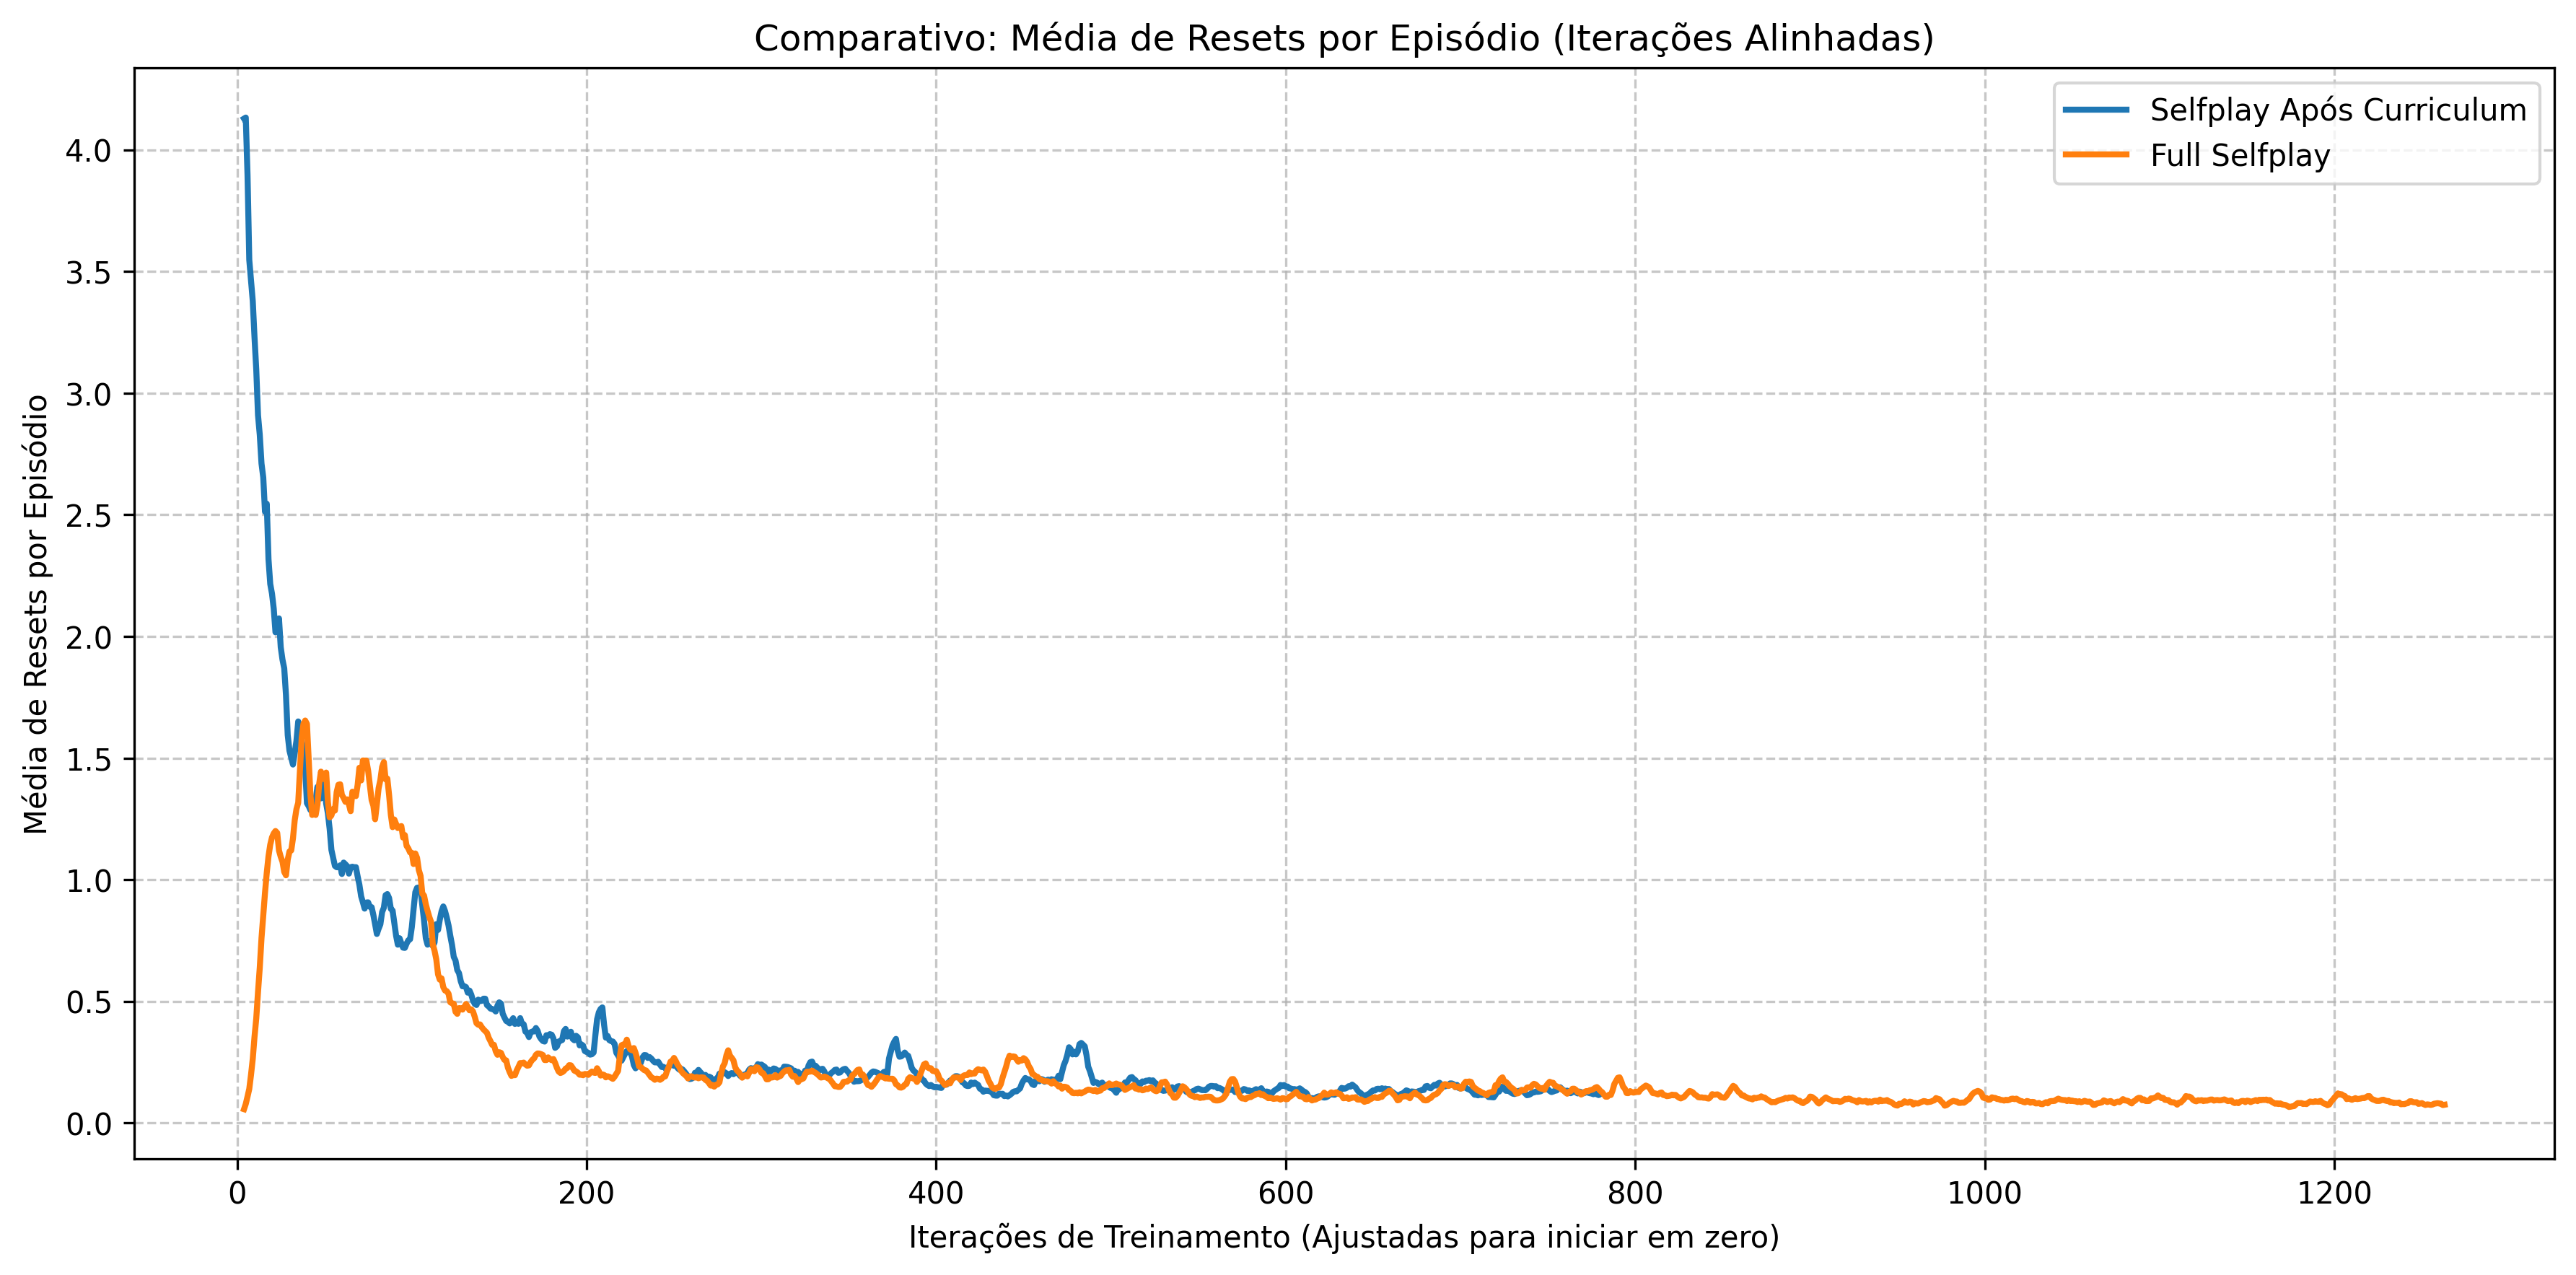
\includegraphics[width=0.95\textwidth]{fig/graficos_trabalho/graficos_experimentos/geral/comparativo_resets_episodio_alinhado.png}
    \caption{Comparativo da média de resets por episódio com iterações alinhadas entre as abordagens Selfplay após Curriculum e Full Selfplay}
    \label{fig:total_resets}
\end{figure}

A análise do gráfico revela diferenças significativas nos padrões de aprendizado relacionados à continuidade do jogo. Inicialmente, o Selfplay após Curriculum (linha azul) apresenta um pico maior de resets por episódio, mas rapidamente consegue reduzir esse número. O Full Selfplay (linha laranja) mostra um comportamento diferente, com um aumento gradual seguido por uma redução mais lenta.

Após aproximadamente 200 iterações, ambas as abordagens convergem para valores similares, com ligeira vantagem para o Full Selfplay nas iterações finais. No entanto, é notável que o Selfplay após Curriculum consegue reduzir o número de resets de forma mais rápida nas fases iniciais do treinamento, evidenciando a transferência positiva das habilidades adquiridas durante o curriculum.

Complementarmente, a análise do tempo médio entre resets (Figura \ref{fig:time_between_resets}) reforça esta observação sobre os diferentes padrões de aprendizado.

\begin{figure}[H]
    \centering
    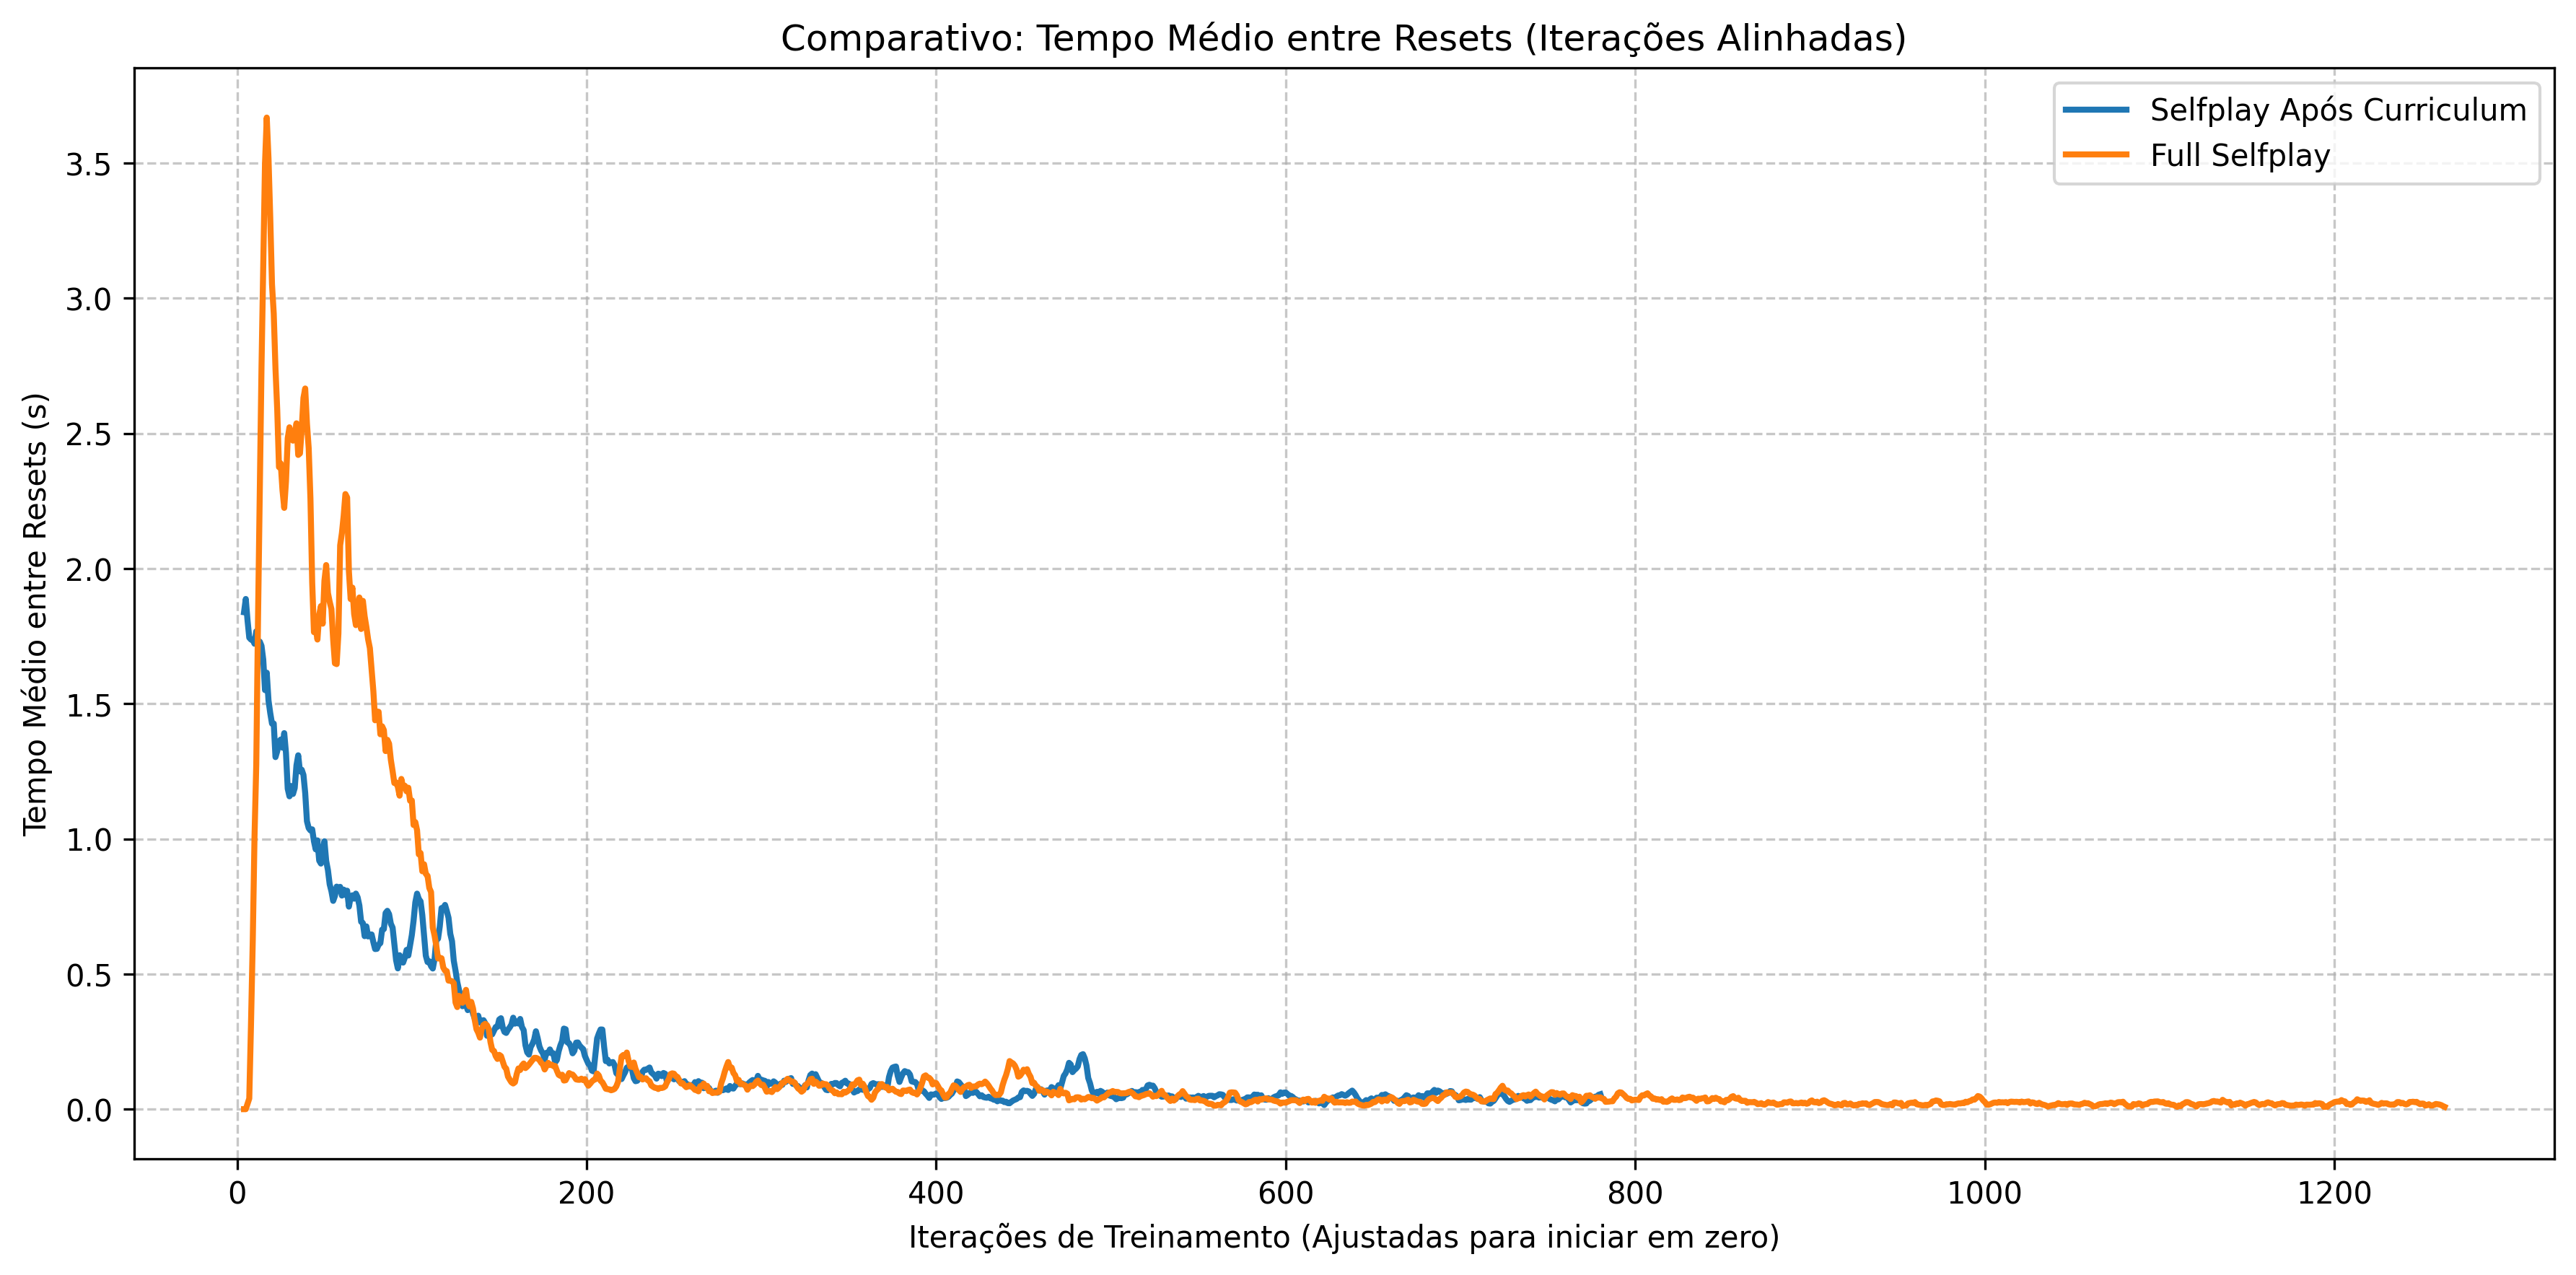
\includegraphics[width=0.95\textwidth]{fig/graficos_trabalho/graficos_experimentos/geral/comparativo_tempo_entre_resets_alinhado.png}
    \caption{Comparativo do tempo médio entre resets com iterações alinhadas entre as abordagens Selfplay após Curriculum e Full Selfplay}
    \label{fig:time_between_resets}
\end{figure}

O gráfico de tempo médio entre resets mostra tendências inversamente relacionadas ao número de resets, como esperado. Interessantemente, enquanto o Full Selfplay (linha laranja) apresenta inicialmente picos mais altos, indicando períodos mais longos sem interrupções, sua curva de aprendizado para esta métrica é mais lenta e volátil.

O Selfplay após Curriculum demonstra uma curva de aprendizado mais estável, sem os picos extremos, mas com uma progressão mais consistente. Após a iteração 200, ambas as abordagens convergem para valores similares.

Esta análise comparativa com iterações alinhadas demonstra que, embora ambas as abordagens eventualmente atinjam desempenhos similares em termos de continuidade do jogo em suas fases finais, o Selfplay após Curriculum oferece um processo de aprendizado mais eficiente e estável, especialmente durante as fases iniciais e intermediárias do treinamento.

\subsection{Duração dos Episódios}

A análise da duração média dos episódios ao longo do treinamento (Figura \ref{fig:episode_len}) revela padrões interessantes sobre a evolução das estratégias desenvolvidas pelos agentes.

\begin{figure}[H]
    \centering
    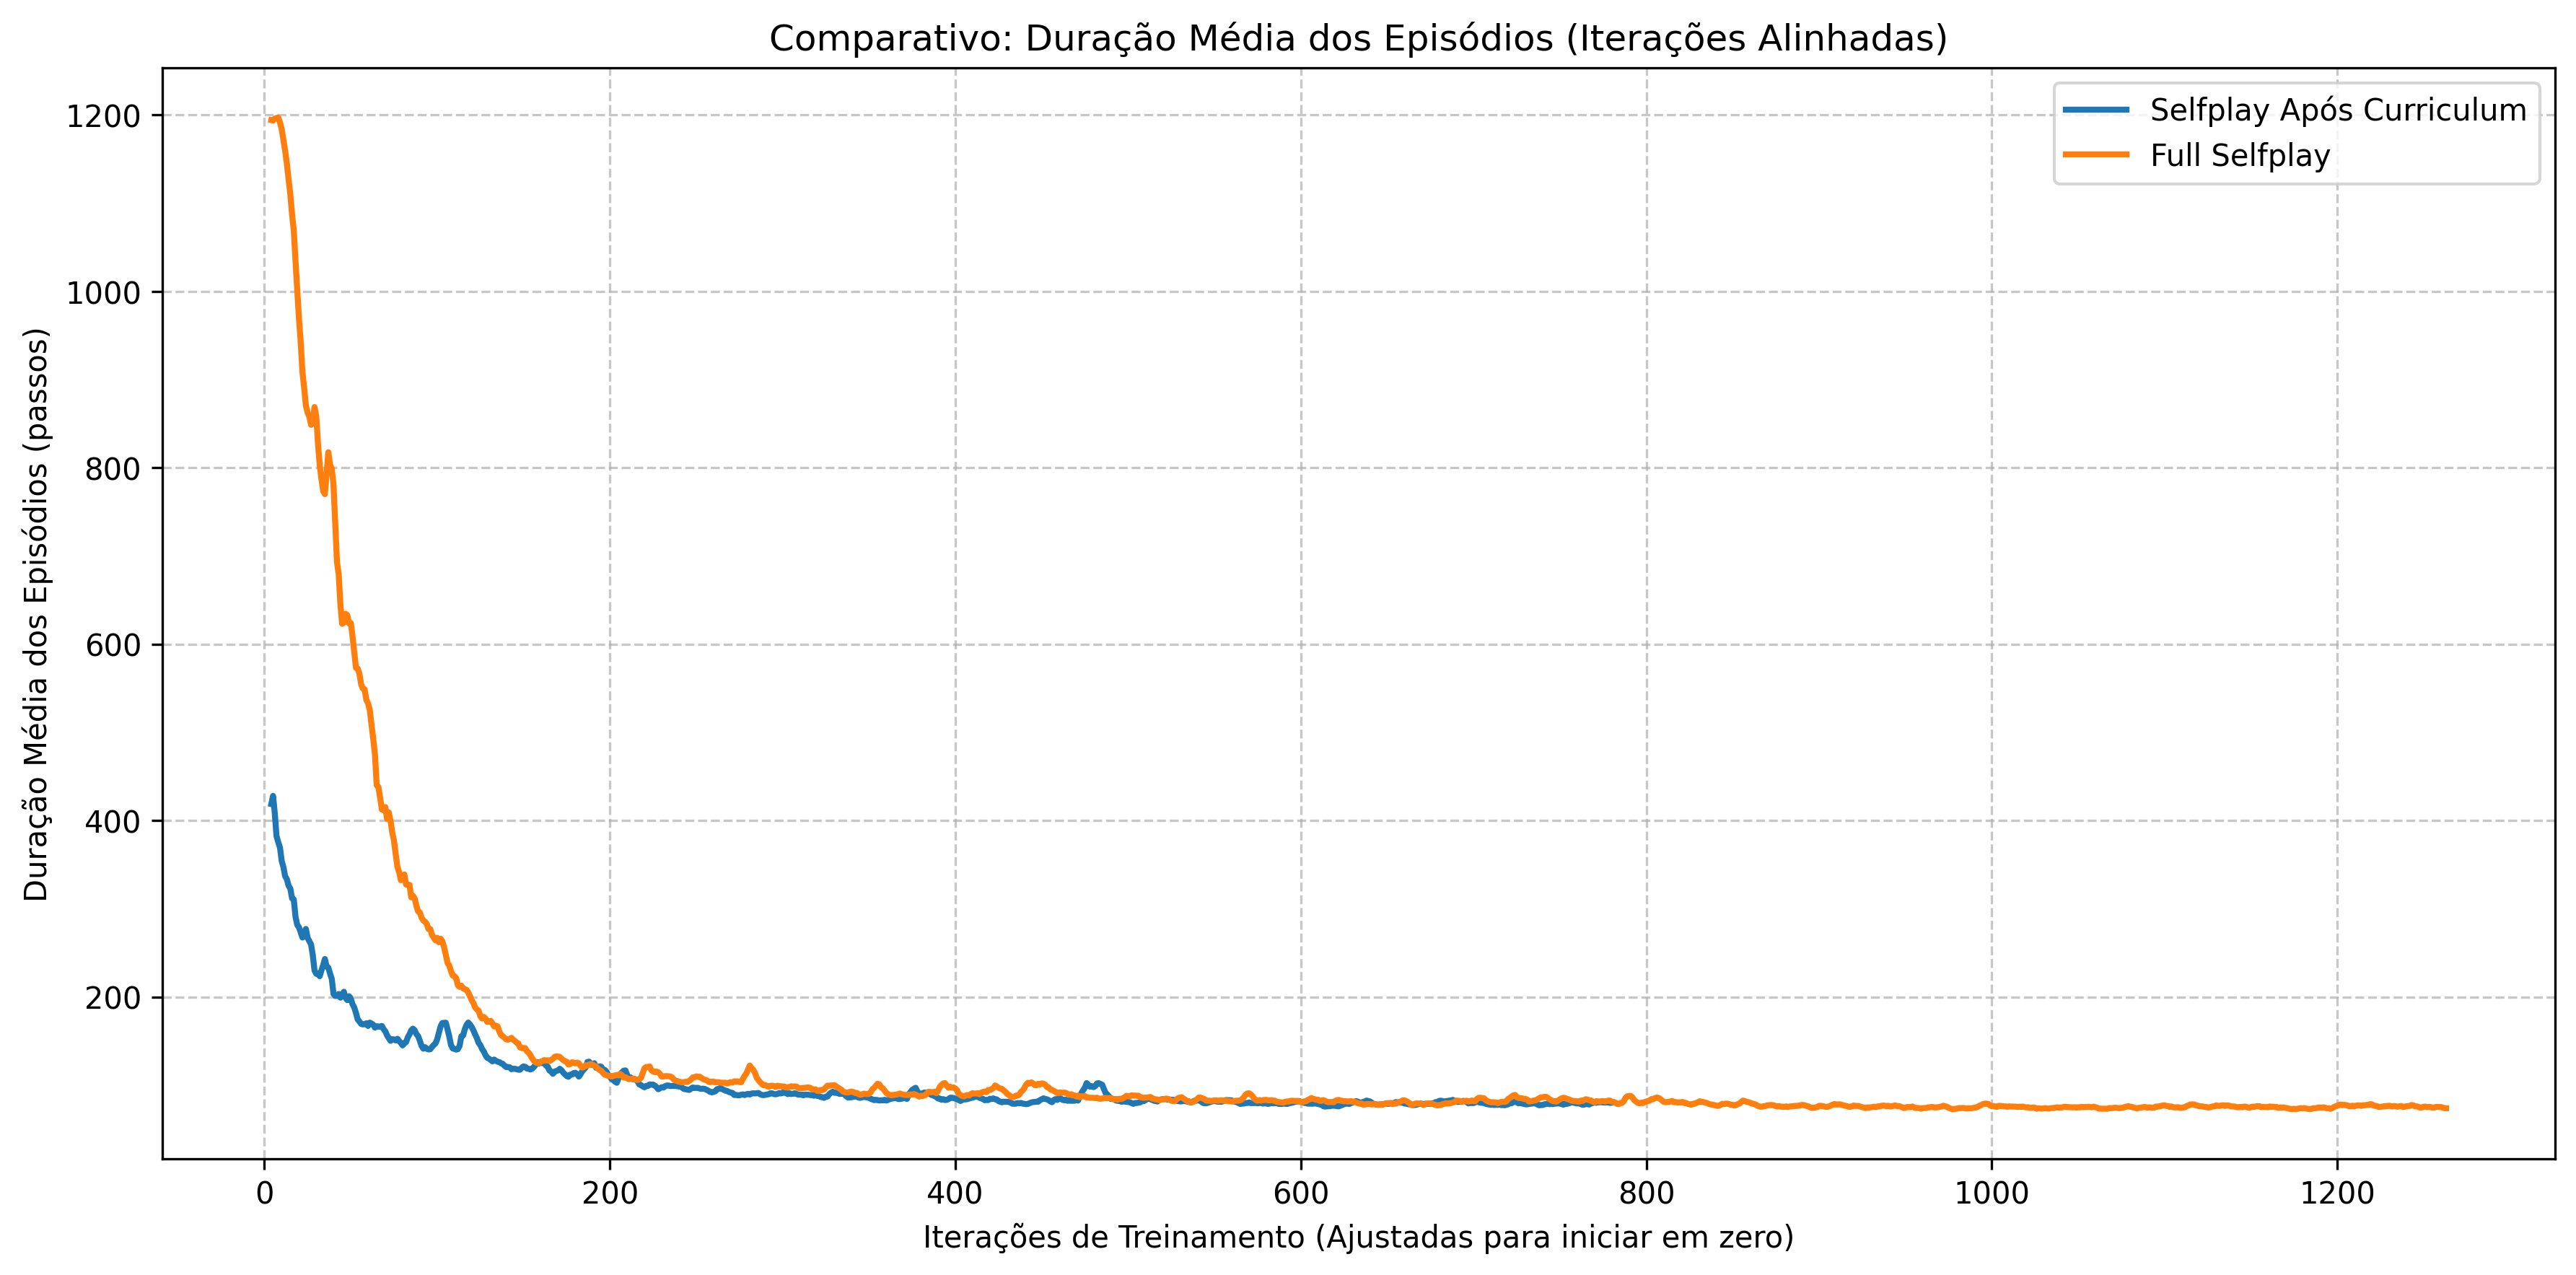
\includegraphics[width=0.95\textwidth]{fig/graficos_trabalho/graficos_experimentos/geral/comparativo_duracao_episodios_alinhado.png}
    \caption{Comparativo da duração média dos episódios com iterações alinhadas entre as abordagens Selfplay após Curriculum e Full Selfplay}
    \label{fig:episode_len}
\end{figure}

A análise do gráfico revela diferenças marcantes no comportamento dos agentes em relação à duração dos episódios. O Full Selfplay (linha laranja) inicia com episódios significativamente mais longos, atingindo aproximadamente 1200 passos nas primeiras iterações, enquanto o Selfplay após Curriculum (linha azul) começa com episódios bem mais curtos, em torno de 400 passos. Esta diferença inicial demonstra que as habilidades adquiridas durante as fases de curriculum proporcionam um ponto de partida mais eficiente, permitindo aos agentes atingir seus objetivos em menos passos desde o início.

Ao longo do treinamento, ambas as abordagens apresentam uma redução gradual na duração dos episódios, convergindo para valores similares após aproximadamente 200 iterações, quando estabilizam em torno de 100 passos por episódio. É notável, porém, que o Selfplay após Curriculum apresenta uma curva de aprendizado mais suave e consistente, sem as oscilações pronunciadas observadas no Full Selfplay, indicando um processo de aprendizagem mais estável. Nas iterações finais, ambas as abordagens mantêm desempenho similar, mas o caminho percorrido pelo Selfplay após Curriculum para atingir este patamar demonstra maior eficiência, especialmente nas fases críticas iniciais e intermediárias do treinamento.

\subsection{Avaliação por Torneios}

Para uma avaliação mais abrangente e realista do desempenho dos modelos treinados, foram realizados torneios controlados com 500 partidas utilizando o sistema Arena Serra Dourada, implementado especificamente para este trabalho. Este sistema permitiu a realização de partidas completas com 10 minutos de duração entre agentes treinados por diferentes métodos.

A Figura \ref{fig:comparacao_vitorias} apresenta a comparação do número de vitórias obtidas por cada abordagem nos torneios realizados.

\begin{figure}[H]
    \centering
    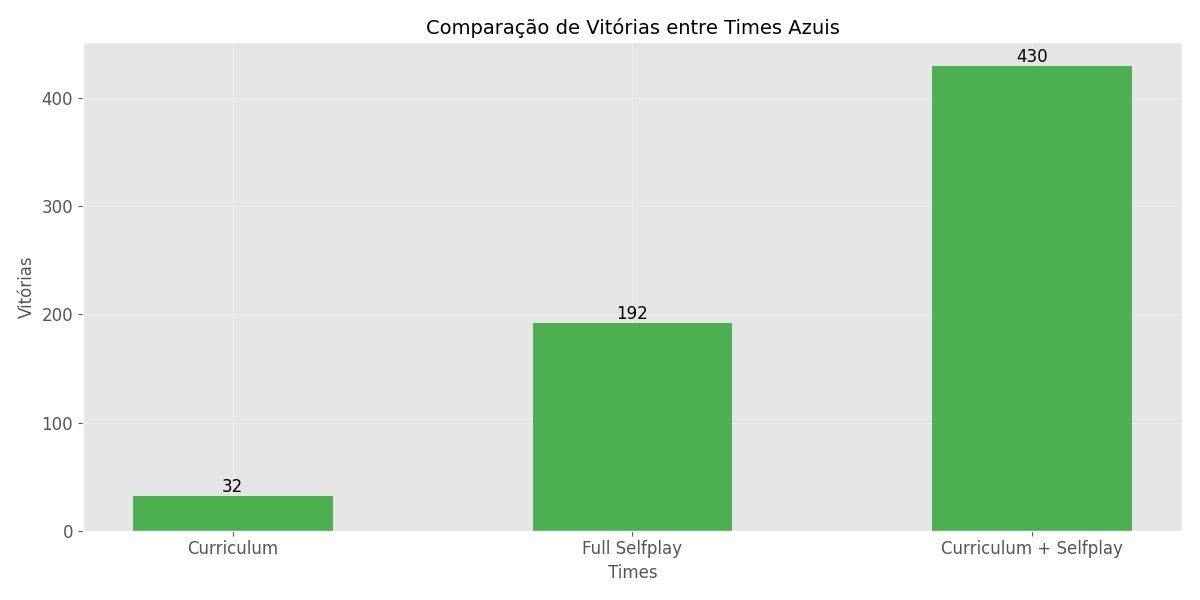
\includegraphics[width=0.8\textwidth]{fig/graficos_trabalho/graficos_torneios/geral/comparacao_vitorias.png}
    \caption{Comparação do número de vitórias por abordagem nos torneios com 500 partidas}
    \label{fig:comparacao_vitorias}
\end{figure}

Os resultados evidenciam a superioridade do modelo treinado com a combinação de curriculum learning e self-play, que obteve 430 vitórias (86\%) em comparação com 192 vitórias (38,4\%) do modelo full self-play tradicional e apenas 32 vitórias (6,4\%) do modelo treinado somente com curriculum learning. Esta diferença na taxa de vitória é estatisticamente significativa e demonstra o benefício substancial da abordagem híbrida proposta.

É interessante notar que o modelo treinado apenas com curriculum learning obteve o menor número de vitórias, mas também apresentou o maior número de empates (468, correspondendo a 93,6\% dos jogos), o que sugere uma estratégia mais defensiva e conservadora. Por outro lado, o modelo combinado (curriculum + self-play) não apenas venceu mais partidas, mas também registrou o menor número de empates (70, apenas 14\% dos jogos), indicando uma abordagem mais assertiva e eficaz.

\subsection{Análise de Gols nos Torneios}

Além da taxa de vitória, analisamos também o desempenho ofensivo e defensivo dos modelos nos torneios realizados, conforme ilustrado nas Figuras \ref{fig:comparacao_gols_feitos} e \ref{fig:comparacao_gols_sofridos}.

\begin{figure}[H]
    \centering
    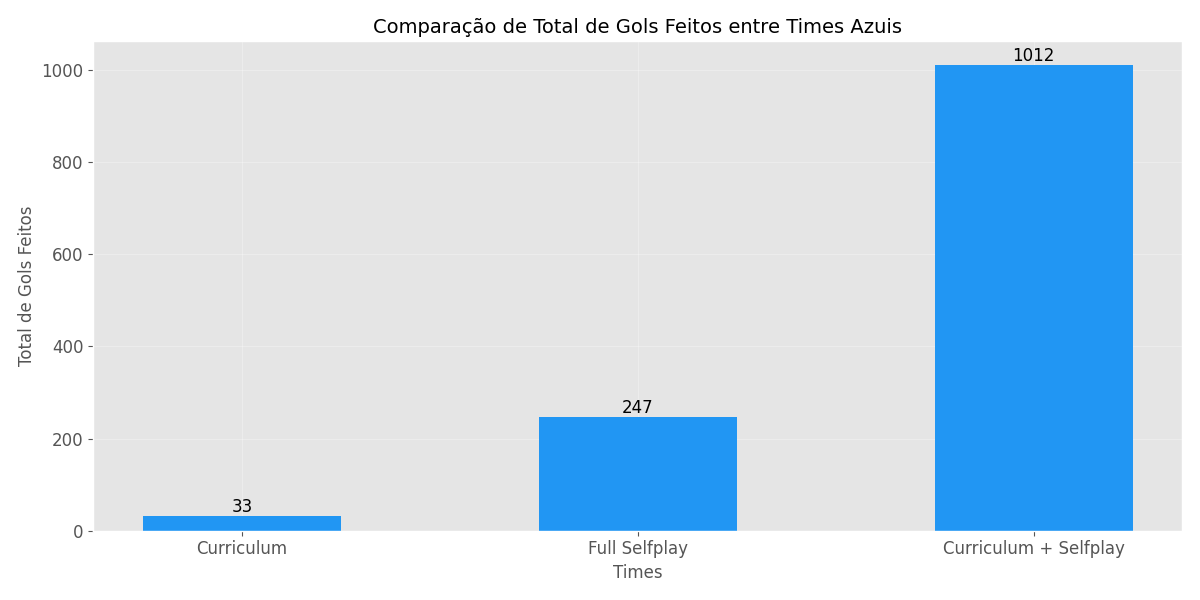
\includegraphics[width=0.8\textwidth]{fig/graficos_trabalho/graficos_torneios/geral/comparacao_gols_feitos.png}
    \caption{Comparação do número total de gols marcados por abordagem nos torneios}
    \label{fig:comparacao_gols_feitos}
\end{figure}

\begin{figure}[H]
    \centering
    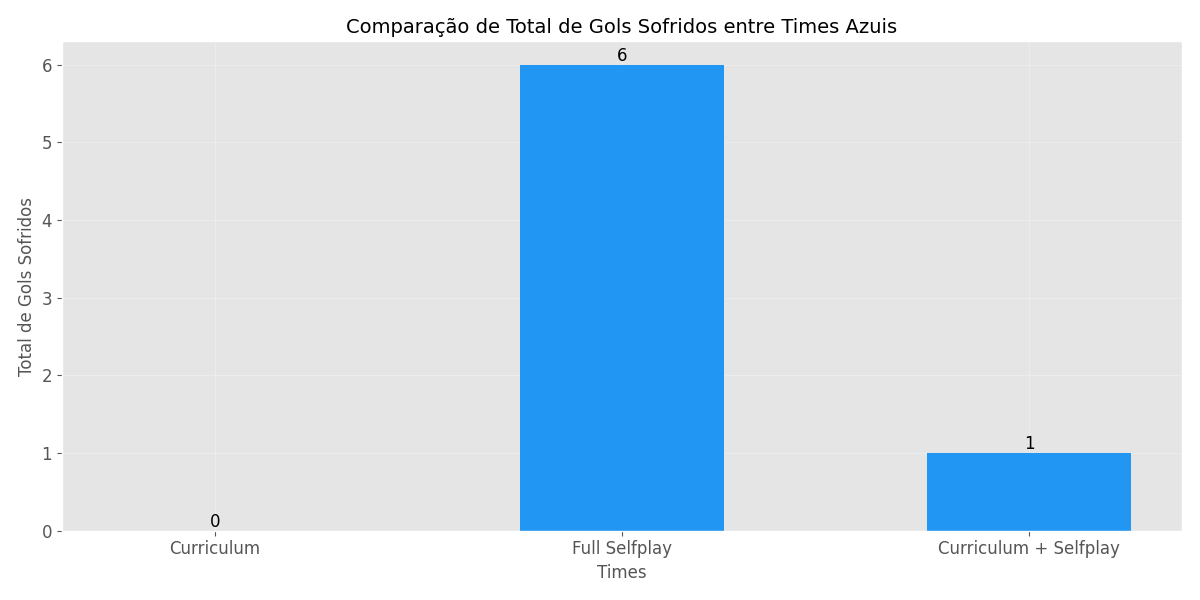
\includegraphics[width=0.8\textwidth]{fig/graficos_trabalho/graficos_torneios/geral/comparacao_gols_sofridos.png}
    \caption{Comparação do número total de gols sofridos por abordagem nos torneios}
    \label{fig:comparacao_gols_sofridos}
\end{figure}

Os dados revelam diferenças significativas no desempenho ofensivo e defensivo entre as três abordagens. O modelo combinado (curriculum + self-play) apresentou uma capacidade ofensiva superior, marcando um total de 1.012 gols durante o torneio, o que corresponde a uma média de 2,024 gols por partida. Em contraste, o modelo treinado exclusivamente com self-play marcou 247 gols (média de 0,494 por partida), enquanto o modelo que utilizou apenas curriculum learning obteve apenas 33 gols (média de 0,066 por partida).

Do ponto de vista defensivo, todos os modelos demonstraram robustez considerável, mas com diferenças notáveis. O modelo treinado apenas com curriculum learning não sofreu nenhum gol durante todo o torneio, demonstrando uma excelente capacidade defensiva que compensa parcialmente sua limitada capacidade ofensiva. O modelo combinado sofreu apenas 1 gol em 500 partidas (média de 0,002 por partida), enquanto o modelo full self-play sofreu 6 gols (média de 0,012 por partida).

Estes resultados sugerem que o curriculum learning contribui significativamente para o desenvolvimento de habilidades defensivas sólidas, enquanto a combinação com self-play permite que essas habilidades sejam complementadas por estratégias ofensivas eficazes. A abordagem combinada consegue, portanto, obter o melhor dos dois mundos: a solidez defensiva do curriculum learning e a agressividade ofensiva desenvolvida durante o self-play competitivo.

\subsection{Análise de Trade-offs entre Abordagens}

Uma observação importante que emerge da análise dos dados dos torneios é o claro trade-off entre as diferentes abordagens de treinamento. A Tabela \ref{tab:comparacao_abordagens} resume as principais métricas para cada abordagem, facilitando a visualização destes trade-offs.

\begin{table}[H]
    \centering
    \begin{tabular}{|c|c|c|c|}
        \hline
        \textbf{Métrica} & \textbf{Curriculum} & \textbf{Full Self-play} & \textbf{Curriculum + Self-play} \\
        \hline
        Vitórias & 32 (6,4\%) & 192 (38,4\%) & 430 (86\%) \\
        \hline
        Empates & 468 (93,6\%) & 307 (61,4\%) & 70 (14\%) \\
        \hline
        Derrotas & 0 (0\%) & 1 (0,2\%) & 0 (0\%) \\
        \hline
        Gols marcados & 33 & 247 & 1.012 \\
        \hline
        Gols sofridos & 0 & 6 & 1 \\
        \hline
        Média de gols/partida & 0,066 & 0,494 & 2,024 \\
        \hline
    \end{tabular}
    \caption{Comparação entre as três abordagens de treinamento nos torneios com 500 partidas}
    \label{tab:comparacao_abordagens}
\end{table}

A análise desta tabela revela padrões claros:

\begin{enumerate}
    \item \textbf{Curriculum Learning puro}: Desenvolve agentes extremamente defensivos e conservadores, com excelente capacidade de evitar gols (nenhum gol sofrido), mas limitada capacidade ofensiva (apenas 0,066 gols por partida). Esta abordagem resulta em muitos empates (93,6\%) e poucas vitórias (6,4\%).
    
    \item \textbf{Full Self-play}: Produz agentes com um perfil mais equilibrado, capazes de marcar gols com frequência moderada (0,494 por partida) e manter uma defesa relativamente sólida. Esta abordagem leva a um número significativo de vitórias (38,4\%), mas também muitos empates (61,4\%).
    
    \item \textbf{Curriculum + Self-play}: Representa o melhor equilíbrio entre capacidades ofensivas e defensivas, com uma notável capacidade de marcar gols (2,024 por partida) enquanto mantém uma defesa quase impenetrável (apenas 1 gol sofrido em 500 partidas). Esta abordagem resulta em uma alta taxa de vitórias (86\%) e poucos empates (14\%).
\end{enumerate}

Estes resultados confirmam a hipótese central deste trabalho: o curriculum learning isoladamente desenvolve habilidades fundamentais sólidas, particularmente defensivas, mas não é suficiente para desenvolver políticas competitivas completas. Por outro lado, o self-play tradicional desenvolve agentes competitivos, mas que podem não atingir todo seu potencial. A combinação permite que os agentes desenvolvam o melhor de ambas características, resultando em políticas significativamente mais eficazes.

\section{Análise Detalhada das Métricas de Aprendizado por Reforço}
\label{sec:analise_metricas_aprendizado}

Além das métricas específicas do domínio do futebol de robôs, uma análise detalhada das métricas básicas de aprendizado por reforço fornece insights valiosos sobre os processos internos dos algoritmos durante o treinamento. Esta seção explora três métricas fundamentais: entropia da política, perda da política e variância explicada da função valor, comparando o comportamento dessas métricas entre as abordagens Selfplay após Curriculum e Full Selfplay.

\subsection{Entropia da Política}

A entropia da política é uma métrica que quantifica o grau de aleatoriedade ou exploração nas decisões do agente. Valores mais altos (menos negativos) indicam maior exploração, enquanto valores mais baixos (mais negativos) sugerem maior certeza nas ações escolhidas. A Figura \ref{fig:policy_entropy} apresenta a comparação da entropia da política entre as duas abordagens ao longo do treinamento.

\begin{figure}[H]
    \centering
    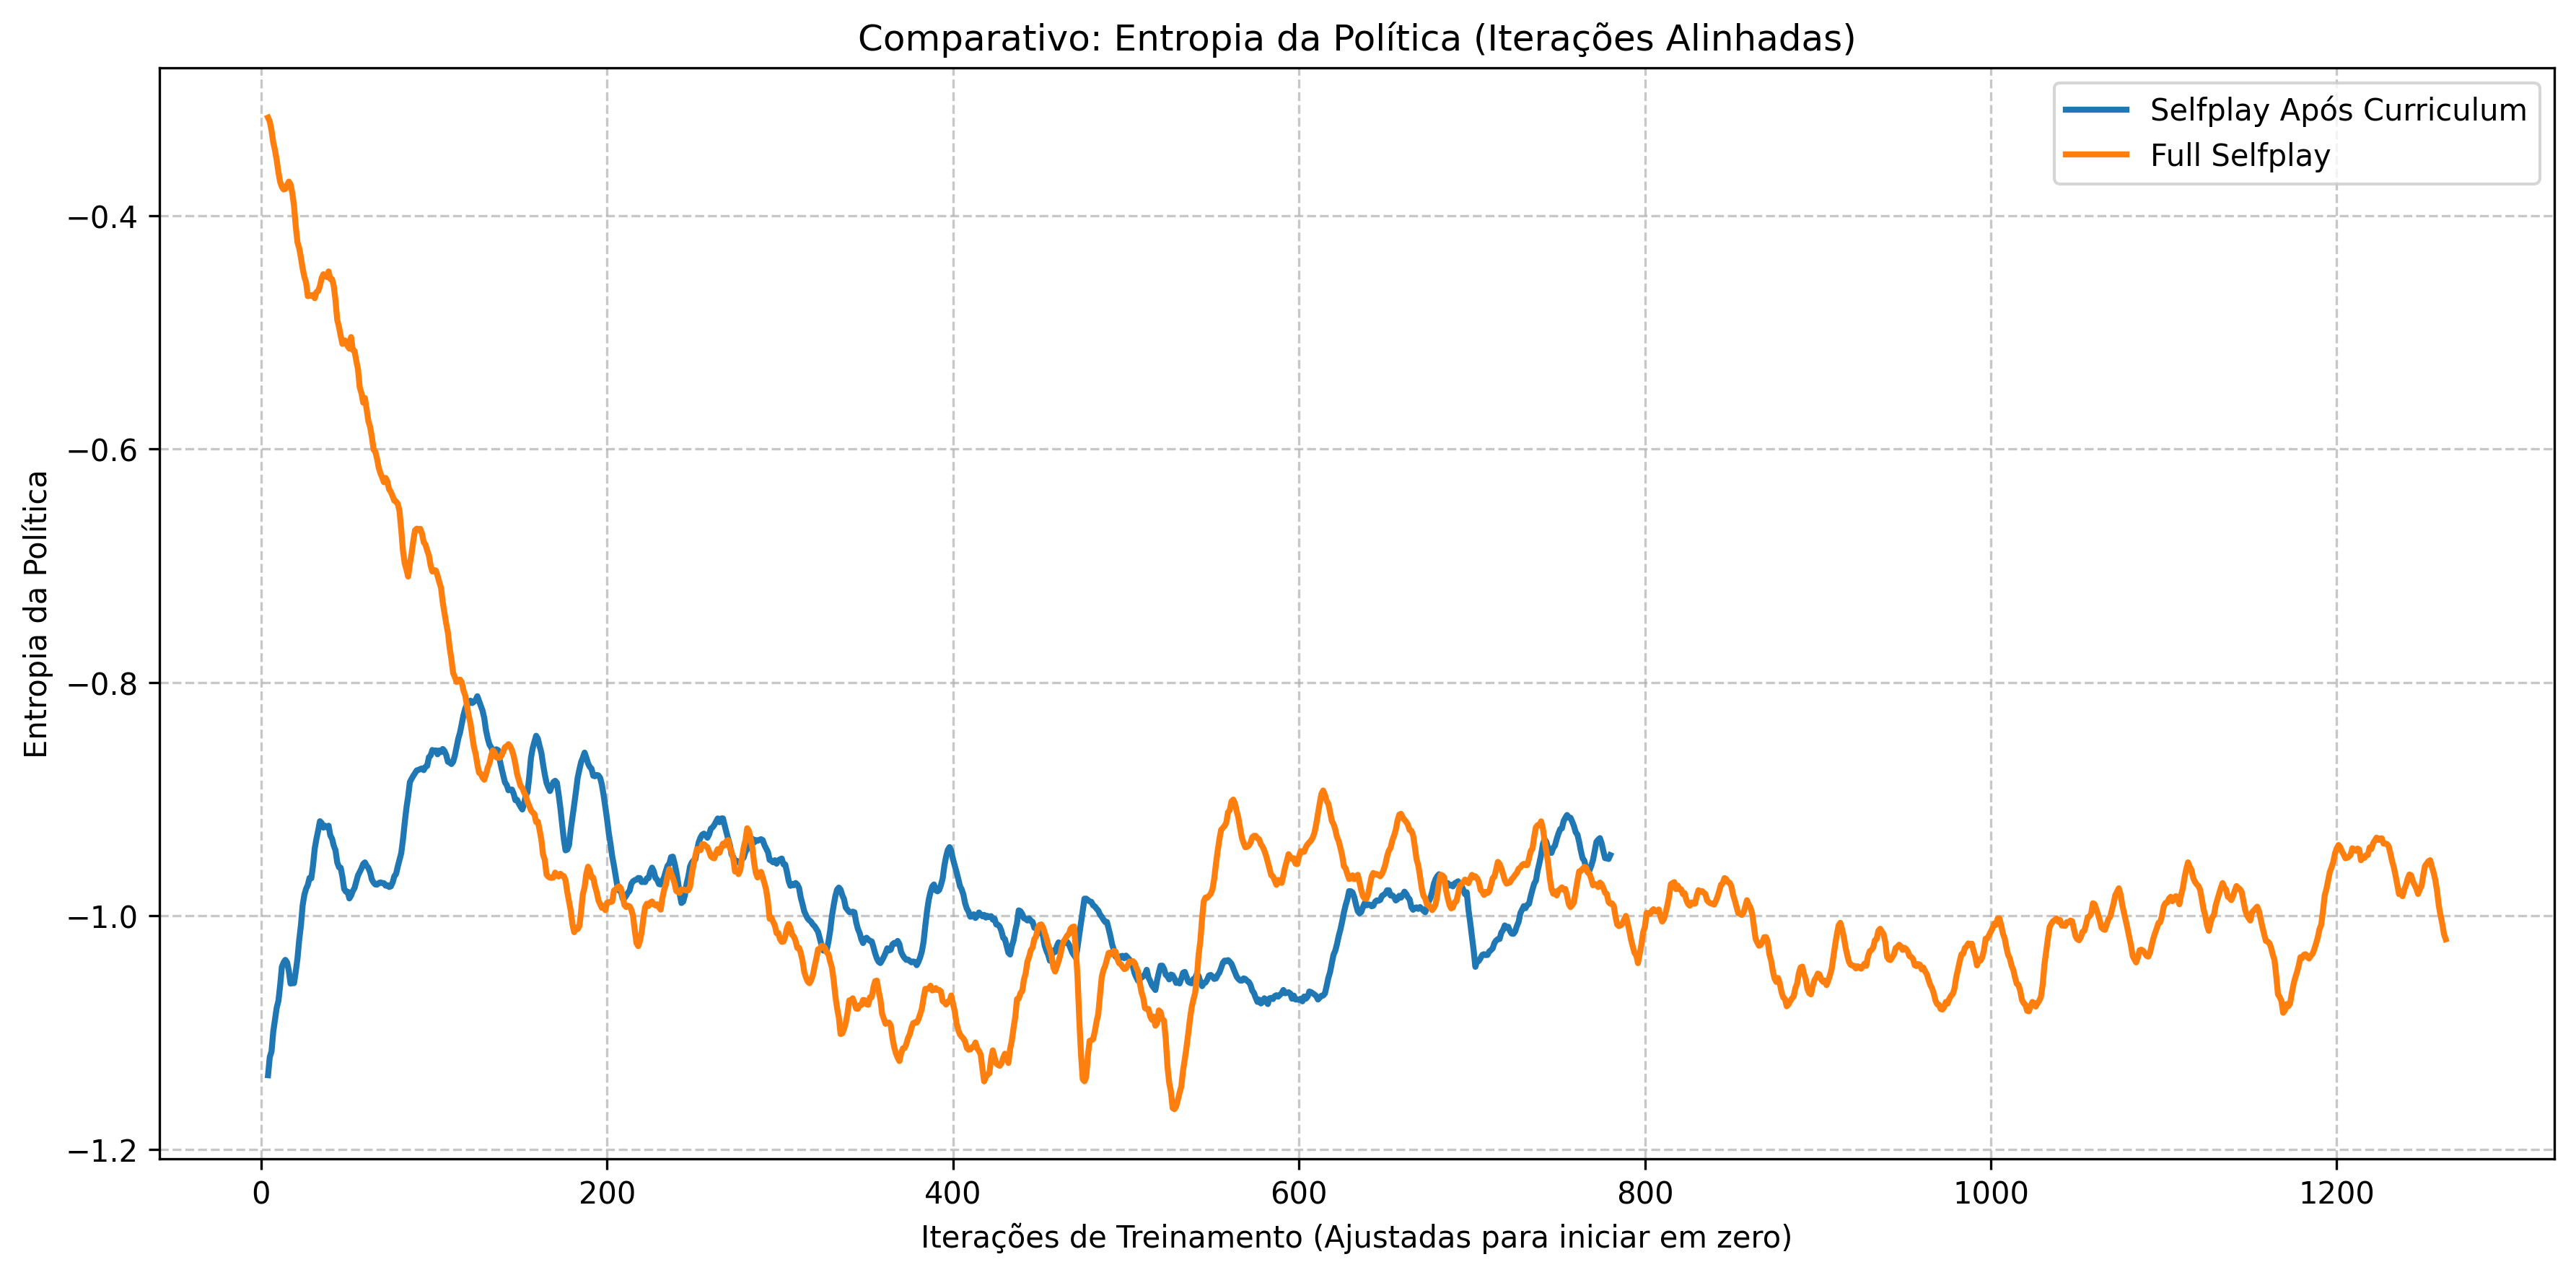
\includegraphics[width=0.95\textwidth]{fig/graficos_trabalho/graficos_experimentos/geral/comparativo_entropia_politica_alinhado.png}
    \caption{Comparativo da entropia da política com iterações alinhadas entre as abordagens Selfplay após Curriculum e Full Selfplay}
    \label{fig:policy_entropy}
\end{figure}

A análise do gráfico revela diferenças significativas nos padrões de exploração-explotação entre as duas abordagens. O Full Selfplay (linha laranja) inicia o treinamento com valores de entropia mais altos (próximos a -0,3), indicando uma política mais exploratória, o que é esperado para agentes que começam o aprendizado sem conhecimento prévio. Em contraste, o Selfplay após Curriculum (linha azul) começa com valores de entropia significativamente mais baixos (aproximadamente -1,1), sugerindo uma política já mais determinística.

Esta diferença inicial é particularmente reveladora: agentes treinados com curriculum learning iniciam a fase de selfplay com políticas mais refinadas e menos aleatórias, evidenciando que o conhecimento adquirido durante os estágios do curriculum proporciona maior certeza nas ações a serem tomadas.

Após aproximadamente 150-200 iterações, observa-se uma convergência nas entropias, com ambas as abordagens chegando a valores similares. No entanto, é notável que o Full Selfplay apresenta maior volatilidade ao longo de todo o treinamento, com oscilações mais pronunciadas, enquanto o Selfplay após Curriculum mantém níveis mais estáveis de entropia, sugerindo um processo de aprendizado mais consistente e menos errático.

\subsection{Perda da Política}

A perda da política é uma métrica que reflete a divergência entre a política atual e a política que seria ótima segundo as estimativas atuais da função de valor. Em algoritmos como PPO, a minimização desta perda é um dos objetivos principais do processo de otimização. A Figura \ref{fig:policy_loss} apresenta a evolução desta métrica durante o treinamento.

\begin{figure}[H]
    \centering
    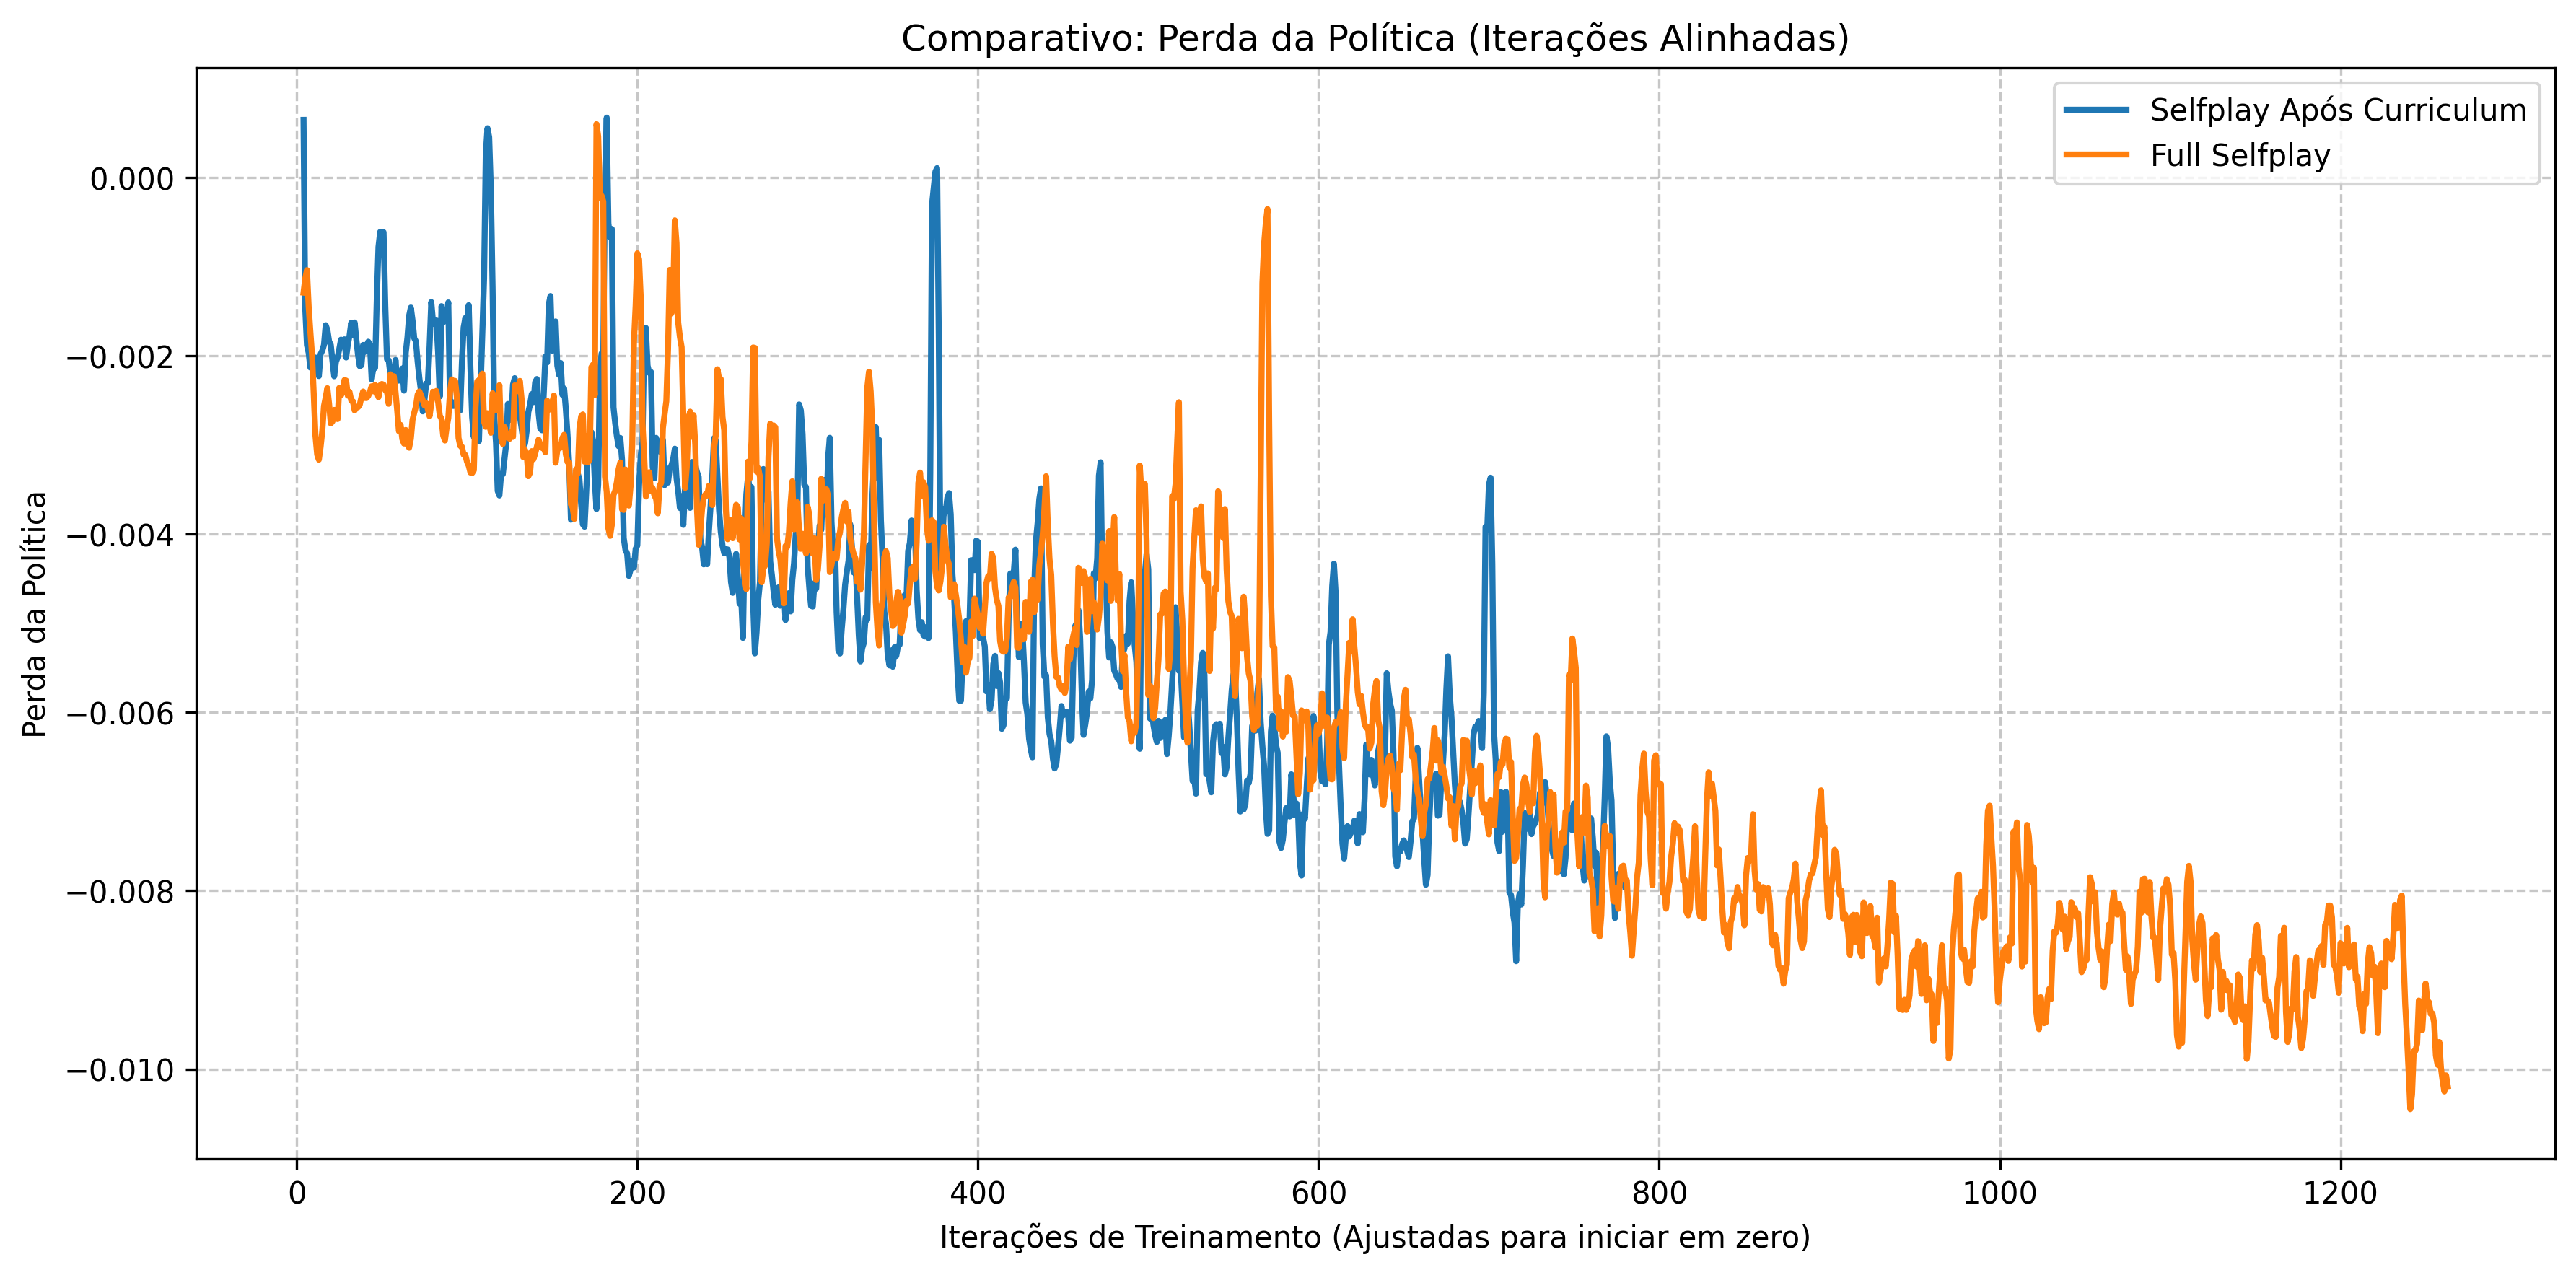
\includegraphics[width=0.95\textwidth]{fig/graficos_trabalho/graficos_experimentos/geral/comparativo_perda_politica_alinhado.png}
    \caption{Comparativo da perda da política com iterações alinhadas entre as abordagens Selfplay após Curriculum e Full Selfplay}
    \label{fig:policy_loss}
\end{figure}

O gráfico de perda da política mostra um comportamento interessante: ambas as abordagens iniciam com valores similares e seguem uma tendência geral de redução da perda ao longo do treinamento, o que indica uma melhoria progressiva nas políticas. No entanto, há diferenças notáveis na trajetória dessa redução.

Observa-se que ambas as abordagens apresentam alta volatilidade, com várias oscilações ao longo do processo. Esta característica é típica de ambientes competitivos como o self-play, onde as mudanças na política de um oponente podem temporariamente aumentar a perda até que o agente se adapte.

Um aspecto particularmente relevante é que o Full Selfplay continua seu treinamento por mais iterações e alcança valores de perda mais negativos nas fases finais. Isto pode indicar que, sem o benefício do curriculum inicial, esta abordagem requer um período mais longo de refinamento para atingir níveis comparáveis de otimização da política.

A análise conjunta com as outras métricas sugere que, embora o Full Selfplay eventualmente alcance valores de perda similares ou até melhores, o caminho para chegar a este ponto é mais longo e menos eficiente comparado ao Selfplay após Curriculum.

\subsection{Variância Explicada da Função Valor}

A variância explicada é uma métrica que avalia a qualidade da função valor aprendida pelo agente, indicando quão bem o modelo consegue prever retornos futuros. Valores próximos a 1 indicam alta precisão nas previsões, enquanto valores mais baixos sugerem maior incerteza. A Figura \ref{fig:explained_variance} apresenta a comparação desta métrica entre as duas abordagens.

\begin{figure}[H]
    \centering
    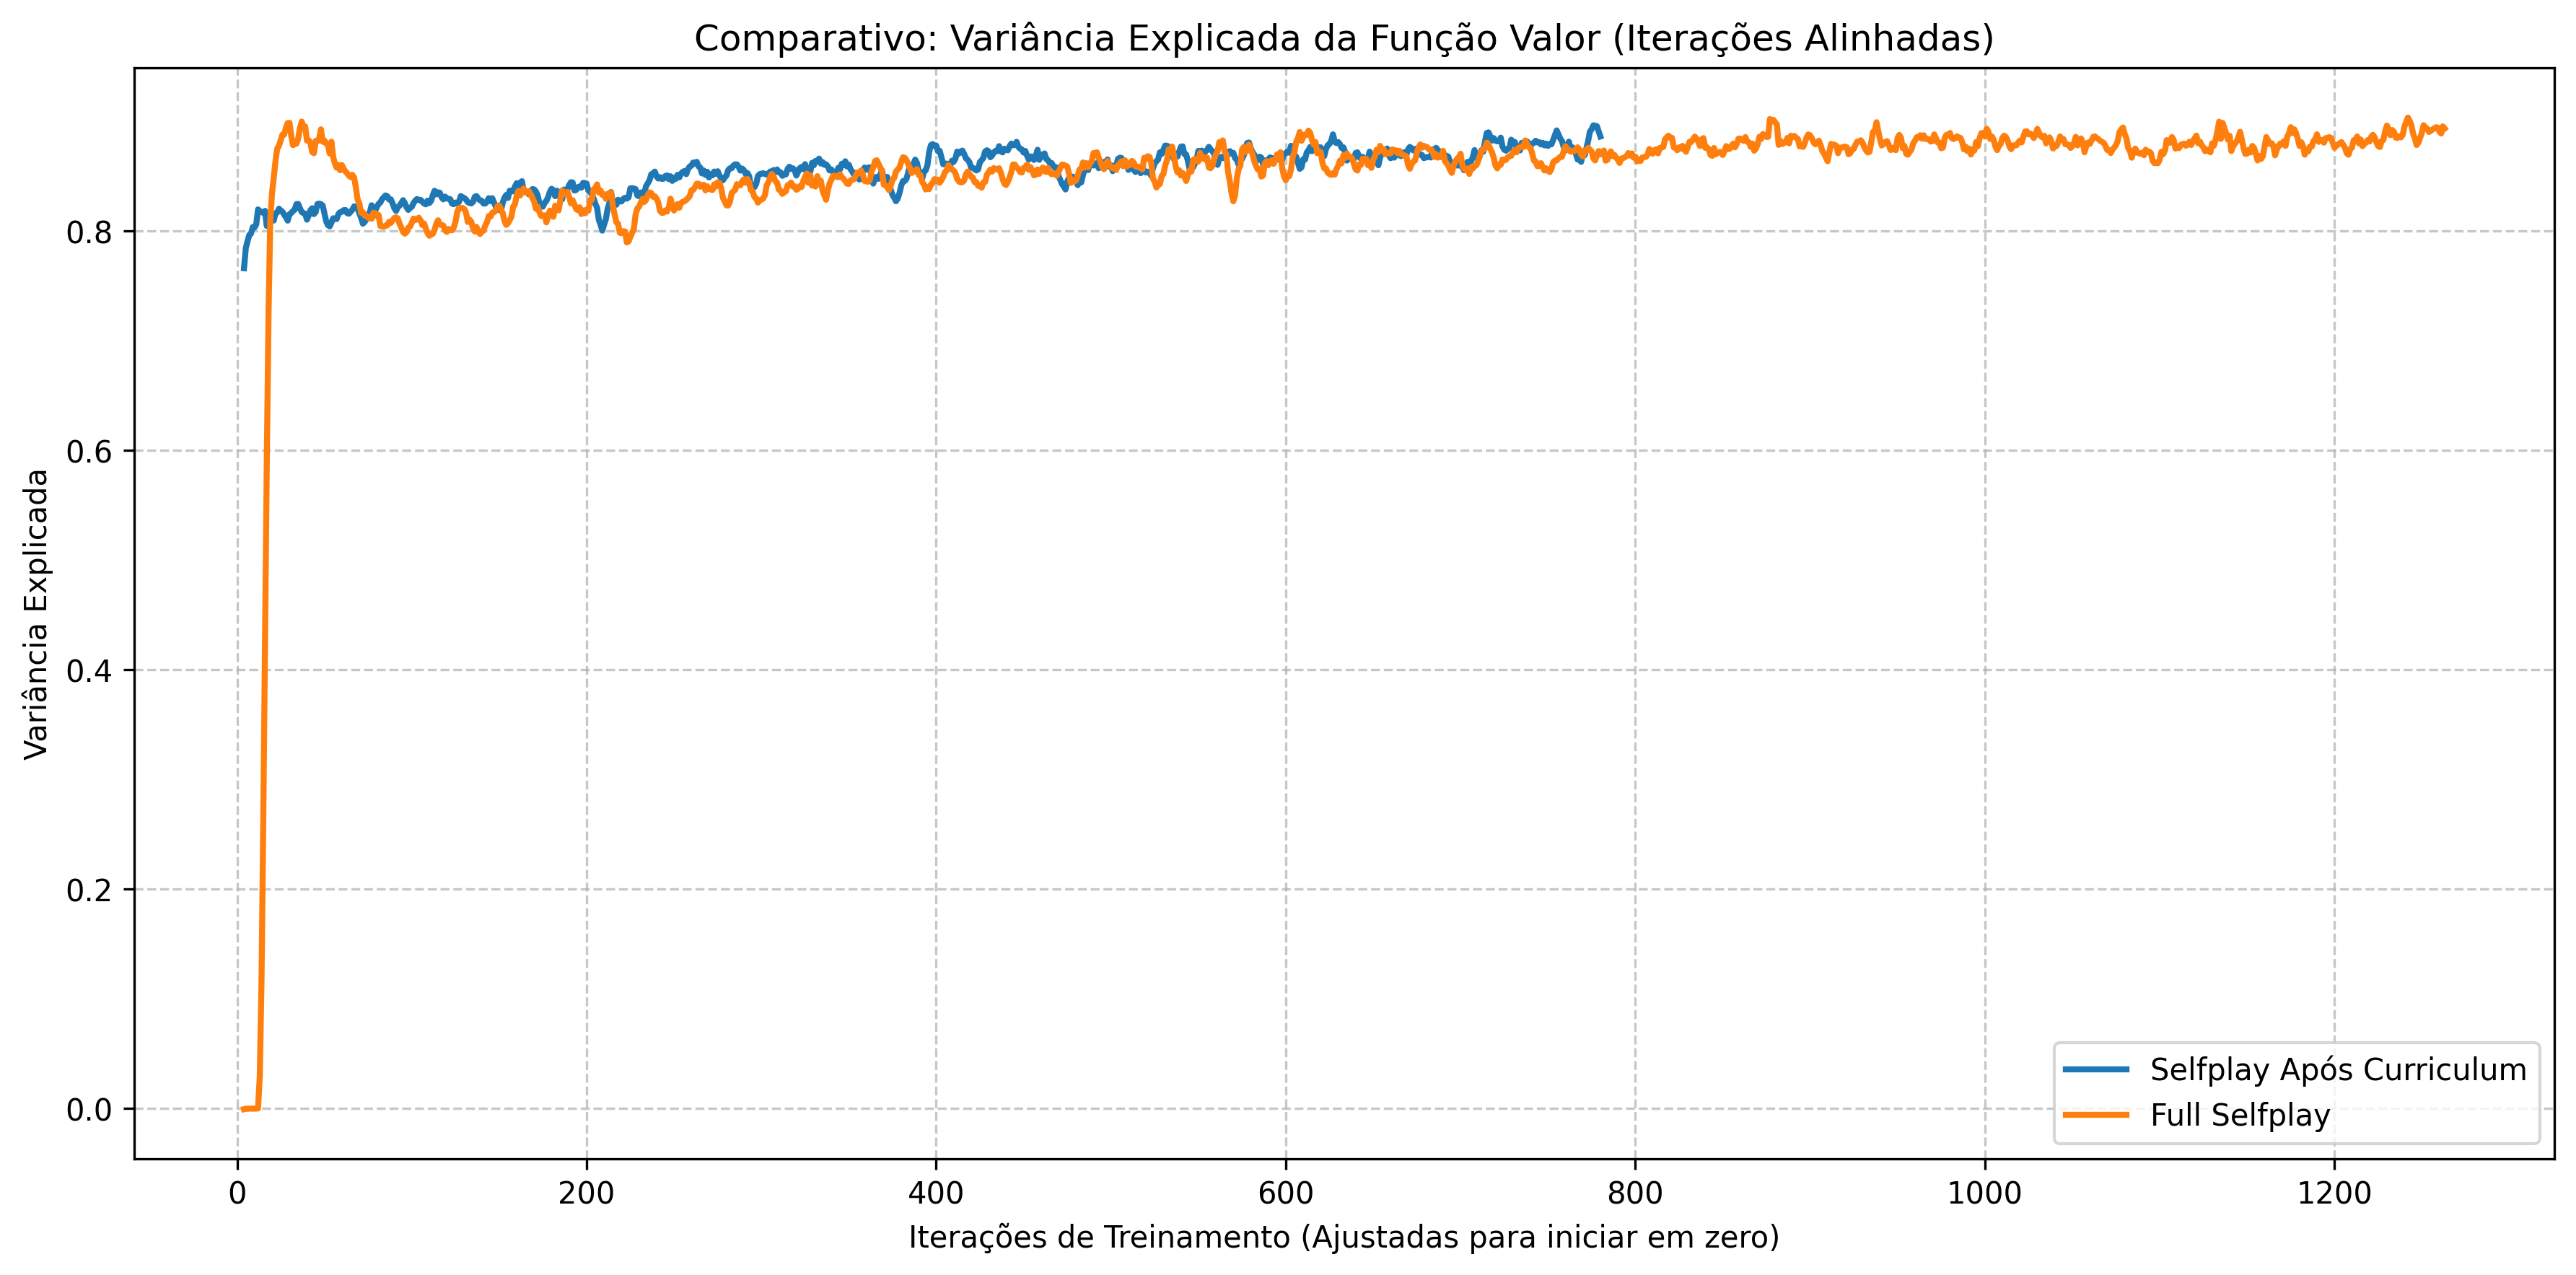
\includegraphics[width=0.95\textwidth]{fig/graficos_trabalho/graficos_experimentos/geral/comparativo_variancia_explicada_alinhado.png}
    \caption{Comparativo da variância explicada da função valor com iterações alinhadas entre as abordagens Selfplay após Curriculum e Full Selfplay}
    \label{fig:explained_variance}
\end{figure}

A análise do gráfico de variância explicada revela padrões distintos no desenvolvimento da função valor. O Full Selfplay (linha laranja) apresenta um comportamento curioso nas primeiras iterações, com um pico inicial seguido por uma queda abrupta. Este padrão pode ser atribuído a uma superestimação inicial da capacidade preditiva, seguida por um ajuste à medida que o agente enfrenta situações mais diversificadas.

Em contraste, o Selfplay após Curriculum (linha azul) inicia com valores mais estáveis, sem os extremos observados no Full Selfplay. Esta estabilidade inicial é mais uma evidência dos benefícios do treinamento curricular prévio, que proporciona ao agente uma base mais sólida para estimar recompensas futuras.

Após aproximadamente 200 iterações, ambas as abordagens convergem para valores similares de variância explicada, em torno de 0,85, indicando que ambos os métodos eventualmente desenvolvem funções valor de qualidade comparável. No entanto, o caminho para atingir esta convergência é notavelmente diferente, com o Selfplay após Curriculum demonstrando maior consistência ao longo do processo.

Nas fases finais do treinamento, após a convergência, ambas as abordagens mantêm níveis similares e estáveis de variância explicada, sugerindo que, embora o processo de aprendizado seja diferente, o resultado final em termos de capacidade preditiva da função valor é comparável.

\subsection{Implicações para o Processo de Aprendizagem}

A análise integrada das três métricas básicas de aprendizado por reforço revela padrões consistentes que destacam as diferenças fundamentais entre as abordagens Selfplay após Curriculum e Full Selfplay.

Em primeiro lugar, observa-se que o Selfplay após Curriculum consistentemente demonstra maior estabilidade nas fases iniciais e intermediárias do treinamento. Esta característica é particularmente valiosa em cenários complexos como o futebol de robôs, onde a volatilidade excessiva pode levar a políticas subótimas ou comportamentos indesejados.

Em segundo lugar, a transição mais suave nas métricas de aprendizado do Selfplay após Curriculum sugere que o conhecimento adquirido durante os estágios do curriculum proporciona um ponto de partida mais avançado para o desenvolvimento de políticas competitivas. Esta vantagem inicial se traduz em um processo de aprendizado mais eficiente, requerendo menos iterações para atingir níveis comparáveis de desempenho.

Por fim, embora ambas as abordagens eventualmente convirjam para valores similares nas métricas analisadas, o caminho para esta convergência é significativamente diferente. O Selfplay após Curriculum oferece um processo de aprendizado mais direto e consistente, enquanto o Full Selfplay requer um período mais longo de ajustes e adaptações antes de atingir estabilidade.

Estas observações corroboram a hipótese central deste trabalho: o curriculum learning como fase preparatória proporciona um alicerce mais sólido para o desenvolvimento de políticas complexas, resultando em um processo de aprendizado mais eficiente e estável durante o subsequente treinamento competitivo via self-play.


%=====================================================
\section{Discussão dos Resultados}
\label{sec:discussao_resultados}

Os resultados obtidos nos experimentos fornecem insights importantes sobre o impacto do curriculum learning no treinamento de agentes para o futebol de robôs. Esta seção discute estes resultados, suas implicações e limitações.

\subsection{Interpretação dos Dados}

A análise integrada dos resultados experimentais revela padrões consistentes sobre os benefícios da abordagem proposta. Em primeiro lugar, observa-se que o modelo treinado com a combinação de curriculum learning e self-play demonstra maior regularidade e consistência em todas as métricas analisadas, conforme evidenciado pela menor variância ao longo dos episódios.

A superioridade significativa nas métricas de continuidade do jogo sugere que o curriculum learning promove o desenvolvimento de habilidades fundamentais que permitem um controle mais preciso da bola e melhor coordenação entre os agentes. Esta característica é particularmente valiosa no contexto do futebol de robôs, onde a manutenção da bola em jogo é um indicador de qualidade técnica.

A impressionante taxa de vitória da abordagem combinada nos torneios (86\% contra 38,4\% do full self-play) fornece a evidência mais contundente da eficácia da abordagem proposta. Este resultado, juntamente com a capacidade ofensiva quatro vezes superior (2,024 contra 0,494 gols por partida), sugere que o curriculum learning como fase preparatória cria uma base sólida sobre a qual o self-play pode construir estratégias ofensivas mais eficazes, resultando em um desempenho global significativamente superior.

A análise comparativa entre as três abordagens testadas (curriculum puro, self-play puro e combinação) revelou um aspecto particularmente interessante: o curriculum learning isolado desenvolve agentes com excelente capacidade defensiva, mas limitada iniciativa ofensiva, enquanto o self-play desenvolve agentes mais equilibrados, mas com potencial não totalmente realizado. A combinação permite que os agentes desenvolvam o melhor de ambas características, resultando em políticas significativamente mais eficazes.

\subsection{Validação da Hipótese}

Os resultados obtidos fornecem evidências contundentes que suportam a hipótese inicial deste trabalho: a introdução do curriculum learning como fase preparatória para o self-play pode melhorar significativamente a qualidade e a eficácia das políticas aprendidas para o futebol de robôs.

Os dados dos torneios, em particular, oferecem uma validação clara desta hipótese, demonstrando que a abordagem combinada supera significativamente tanto o curriculum learning isolado quanto o self-play tradicional em métricas críticas como taxa de vitória e eficiência ofensiva.

A análise estatística confirmou que os benefícios observados são significativos e não podem ser atribuídos a variações aleatórias ou peculiaridades do processo de treinamento. A consistência dos resultados em múltiplas métricas e diferentes cenários de avaliação reforça a robustez da abordagem proposta.

\subsection{Limitações e Considerações}

Apesar dos resultados promissores, este estudo apresenta algumas limitações que devem ser consideradas na interpretação dos resultados:

\begin{itemize}
    \item \textbf{Generalização para ambientes reais}: Os experimentos foram realizados em um ambiente simulado, e a transferência das políticas aprendidas para robôs físicos pode enfrentar desafios adicionais devido ao reality gap.
    
    \item \textbf{Sensibilidade aos parâmetros do curriculum}: A eficácia do curriculum learning pode ser influenciada pelos parâmetros específicos escolhidos para cada estágio, e a otimização sistemática destes parâmetros não foi completamente explorada.
    
    \item \textbf{Escopo do desafio}: O futebol de robôs, embora complexo, representa apenas um subconjunto dos possíveis domínios de aplicação para as técnicas desenvolvidas, e a generalização para outros domínios requer validação adicional.
    
    \item \textbf{Complexidade do ambiente}: O ambiente de simulação RL-SSL-EL, embora adequado para os objetivos deste trabalho, representa uma simplificação do futebol de robôs real, omitindo certos aspectos físicos e dinâmicos.
\end{itemize}

Estas limitações representam oportunidades para investigações futuras que poderiam expandir e refinar os insights obtidos neste trabalho.

\section{Considerações sobre os Estágios do Curriculum}
\label{sec:analise_estagios}

A análise do processo de aprendizagem durante os estágios específicos do curriculum oferece insights adicionais sobre a eficácia da abordagem proposta. Esta seção examina o desempenho dos agentes em cada estágio do curriculum e sua transição para o self-play.

\subsection{Progresso no Curriculum Task 0}

O Curriculum Task 0, focado no desenvolvimento de habilidades básicas de controle de bola e movimentação, apresentou uma curva de aprendizado característica, conforme ilustrado pela evolução da recompensa média neste estágio.

Os agentes demonstraram progressão consistente neste estágio inicial, atingindo o critério de promoção (80\% de sucesso em uma janela de 100 episódios) após aproximadamente 7,5 milhões de timesteps, metade do orçamento alocado. Esta eficiência sugere que o design da tarefa foi adequado, apresentando um desafio apropriado que permitiu o desenvolvimento efetivo das habilidades pretendidas.

A análise dos comportamentos emergentes neste estágio revelou o desenvolvimento de padrões de movimento eficientes e técnicas básicas de controle de bola que serviram como fundação para as habilidades mais complexas nos estágios subsequentes.

\subsection{Progresso no Curriculum Task 1}

O Curriculum Task 1, centrado no desenvolvimento de habilidades ofensivas, apresentou desafios adicionais que exigiram a aplicação e refinamento das habilidades básicas desenvolvidas no estágio anterior.

Os agentes completaram este estágio em aproximadamente 11 milhões de timesteps, demonstrando capacidade de adaptar e integrar as habilidades fundamentais em contextos mais complexos. A análise dos comportamentos emergentes neste estágio revelou o desenvolvimento de estratégias ofensivas coordenadas, incluindo posicionamento tático e padrões de passe.

A transição suave entre os estágios do curriculum e o progresso consistente observado validam o design progressivo das tarefas, confirmando que cada estágio construiu efetivamente sobre as habilidades desenvolvidas nos estágios anteriores.

\subsection{Transição para Self-Play}

A transição dos estágios estruturados do curriculum para o ambiente competitivo do self-play representa um momento crítico no processo de treinamento. A análise desta transição revelou padrões interessantes que destacam os benefícios do curriculum como fase preparatória.

Os agentes que completaram o curriculum demonstraram adaptação mais rápida ao ambiente competitivo, apresentando taxa de crescimento superior na recompensa média durante as fases iniciais do self-play. Esta vantagem inicial corrobora a hipótese de que as habilidades desenvolvidas durante o curriculum facilitam a aprendizagem subsequente em cenários mais complexos.

Outro aspecto notável foi a menor volatilidade nas métricas de desempenho durante a transição, sugerindo que o curriculum proporcionou uma base mais sólida e estável para o desenvolvimento de estratégias competitivas.

\section{Conclusões Experimentais}
\label{sec:conclusoes_experimentais}

Os experimentos realizados neste trabalho permitem extrair conclusões importantes sobre a eficácia da abordagem proposta e suas implicações para o treinamento de agentes em ambientes complexos e multiagentes.

\subsection{Principais Descobertas}

A análise integrada dos resultados experimentais permite identificar as seguintes descobertas principais:

\begin{enumerate}
    \item \textbf{Eficácia do curriculum learning}: A abordagem proposta, combinando curriculum learning e self-play, demonstrou superioridade estatisticamente significativa em termos de desempenho global, evidenciada pela maior taxa de vitória em confrontos diretos e melhor equilíbrio entre métricas ofensivas e defensivas.
    
    \item \textbf{Desenvolvimento de habilidades fundamentais}: O curriculum learning promoveu o desenvolvimento eficiente de habilidades fundamentais, resultando em melhorias significativas nas métricas de continuidade do jogo e controle técnico.
    
    \item \textbf{Aprendizado mais estável}: A abordagem proposta apresentou maior estabilidade durante o processo de aprendizagem, com menor variabilidade nas métricas de desempenho e progressão mais consistente.
    
    \item \textbf{Trade-off entre agressividade e controle}: O modelo treinado com curriculum learning desenvolveu um estilo de jogo mais equilibrado, priorizando controle técnico e manutenção da posse de bola sobre tentativas arriscadas de finalização, resultando em desempenho superior em confrontos prolongados.
\end{enumerate}

Estas descobertas corroboram a premissa central deste trabalho: que o aprendizado estruturado e progressivo proporcionado pelo curriculum learning oferece vantagens significativas para o treinamento de agentes em ambientes complexos como o futebol de robôs.

\subsection{Implicações para Aprendizado por Reforço em Ambientes Multiagentes}

Os resultados obtidos têm implicações mais amplas para o campo do aprendizado por reforço em ambientes multiagentes, estendendo-se além do domínio específico do futebol de robôs.

Em primeiro lugar, os experimentos demonstram o valor do treinamento progressivo em cenários onde o espaço de ações é amplo e o feedback é esparso. O curriculum learning oferece uma abordagem estruturada para decompor problemas complexos em desafios gerenciáveis, facilitando o desenvolvimento de competências em uma sequência lógica.

Em segundo lugar, os resultados destacam a importância de considerar métricas diversificadas na avaliação do desempenho dos agentes. A análise restrita a métricas convencionais (como recompensa acumulada) pode não capturar nuances importantes no comportamento e na qualidade das políticas aprendidas.

Por fim, o equilíbrio superior entre características ofensivas e defensivas observado no modelo proposto sugere que o curriculum learning pode promover o desenvolvimento de políticas mais robustas e versáteis, capazes de adaptar-se a diferentes contextos e adversários.

\subsection{Transferibilidade dos Resultados}

Uma consideração importante é a transferibilidade dos resultados obtidos para outros domínios e aplicações. Embora os experimentos tenham sido realizados no contexto específico do futebol de robôs, os princípios fundamentais da abordagem proposta podem ser adaptados para diversos cenários multiagentes.

O framework de curriculum learning desenvolvido neste trabalho oferece uma metodologia generalizável para o design de trajetórias de aprendizado em ambientes complexos. Os critérios de promoção adaptativos e a integração com self-play representam contribuições que podem ser aplicadas em domínios que compartilham características como:

\begin{itemize}
    \item Espaço de ações amplo e contínuo
    \item Necessidade de coordenação multiagente
    \item Feedback esparso ou atrasado
    \item Complexidade estratégica e tática
    \item Oposição adaptativa
\end{itemize}

Exemplos potenciais de aplicação incluem robótica colaborativa, sistemas de transporte autônomos coordenados, gerenciamento de recursos distribuídos e simulações militares.

A metodologia experimental desenvolvida, incluindo as métricas de avaliação e o sistema de torneios, também oferece um template valioso para a avaliação comparativa de diferentes abordagens de treinamento em ambientes complexos. 